%%**************************************************************
%% Vorlage fuer Bachelorarbeiten (o.ä.) der DHBW
%%
%% Autor: Tobias Dreher, Yves Fischer
%% Datum: 06.07.2011
%%
%% Autor: Michael Gruben
%% Datum: 15.05.2013
%%**************************************************************
\documentclass[%
	enabledeprecatedfontcommands,
	pdftex,
	oneside,		% Einseitiger Druck.
	12pt,			% Schriftgroesse
	parskip=half,	% Halbe Zeile Abstand zwischen Absätzen.
	headsepline,	% Linie nach Kopfzeile.
	footsepline,	% Linie vor Fusszeile.
	abstracton,	    % Abstract Überschriften
	ngerman,		% Translator
]{scrreprt}
%!TEX root = ../dokumentation.tex

%
% Nahezu alle Einstellungen koennen hier getaetigt werden
%

\RequirePackage[l2tabu, orthodox]{nag}	% weist in Commandozeile bzw. log auf veraltete LaTeX Syntax hin

\documentclass[%
	pdftex,
	oneside,			% Einseitiger Druck.
	12pt,				% Schriftgroesse
	parskip=half,		% Halbe Zeile Abstand zwischen Absätzen.
%	topmargin = 10pt,	% Abstand Seitenrand (Std:1in) zu Kopfzeile [laut log: unused]
	headheight = 12pt,	% Höhe der Kopfzeile
%	headsep = 30pt,	% Abstand zwischen Kopfzeile und Text Body  [laut log: unused]
	headsepline,		% Linie nach Kopfzeile.
	footsepline,		% Linie vor Fusszeile.
	footheight = 16pt,	% Höhe der Fusszeile
	abstracton,		% Abstract Überschriften
	DIV=calc,		% Satzspiegel berechnen
	BCOR=8mm,		% Bindekorrektur links: 8mm
	headinclude=false,	% Kopfzeile nicht in den Satzspiegel einbeziehen
	footinclude=false,	% Fußzeile nicht in den Satzspiegel einbeziehen
	listof=totoc,		% Abbildungs-/ Tabellenverzeichnis im Inhaltsverzeichnis darstellen
	toc=bibliography,	% Literaturverzeichnis im Inhaltsverzeichnis darstellen
]{scrreprt}	% Koma-Script report-Klasse, fuer laengere Bachelorarbeiten alternativ auch: scrbook

% Einstellungen laden
\usepackage{xstring}
\usepackage[utf8]{inputenc}
\usepackage[T1]{fontenc}

\newcommand{\einstellung}[1]{%
  \expandafter\newcommand\csname #1\endcsname{}
  \expandafter\newcommand\csname setze#1\endcsname[1]{\expandafter\renewcommand\csname#1\endcsname{##1}}
}
\newcommand{\langstr}[1]{\einstellung{lang#1}}

\einstellung{matrikelnr}
\einstellung{titel}
\einstellung{kurs}
\einstellung{datumAbgabe}
\einstellung{firma}
\einstellung{firmenort}
\einstellung{abgabeort}
\einstellung{abschluss}
\einstellung{studiengang}
\einstellung{dhbw}
\einstellung{betreuer}
\einstellung{gutachter}
\einstellung{zeitraum}
\einstellung{arbeit}
\einstellung{autor}
\einstellung{sprache}
\einstellung{schriftart}
\einstellung{seitenrand}
\einstellung{kapitelabstand}
\einstellung{spaltenabstand}
\einstellung{zeilenabstand}
\einstellung{zitierstil}
 % verfügbare Einstellungen
%%%%%%%%%%%%%%%%%%%%%%%%%%%%%%%%%%%%%%%%%%%%%%%%%%%%%%%%%%%%%%%%%%%%%%%%%%%%%%%
%                                   Einstellungen
%
% Hier können alle relevanten Einstellungen für diese Arbeit gesetzt werden.
% Dazu gehören Angaben u.a. über den Autor sowie Formatierungen.
%
%
%%%%%%%%%%%%%%%%%%%%%%%%%%%%%%%%%%%%%%%%%%%%%%%%%%%%%%%%%%%%%%%%%%%%%%%%%%%%%%%


%%%%%%%%%%%%%%%%%%%%%%%%%%%%%%%%%%%% Sprache %%%%%%%%%%%%%%%%%%%%%%%%%%%%%%%%%%%
%% Aktuell sind Deutsch und Englisch unterstützt.
%% Es werden nicht nur alle vom Dokument erzeugten Texte in
%% der entsprechenden Sprache angezeigt, sondern auch weitere
%% Aspekte angepasst, wie z.B. die Anführungszeichen und
%% Datumsformate.
\setzesprache{de} % oder en
%%%%%%%%%%%%%%%%%%%%%%%%%%%%%%%%%%%%%%%%%%%%%%%%%%%%%%%%%%%%%%%%%%%%%%%%%%%%%%%%

%%%%%%%%%%%%%%%%%%%%%%%%%%%%%%%%%%% Angaben  %%%%%%%%%%%%%%%%%%%%%%%%%%%%%%%%%%%
%% Die meisten der folgenden Daten werden auf dem
%% Deckblatt angezeigt, einige auch im weiteren Verlauf
%% des Dokuments.
\setzematrikelnr{2463229}
\setzekurs{20ITA}
\setzetitel{In der Regel haben wir einen zweizeiligen Bachelorthesistitel}
\setzedatumAbgabe{Juni 2023}
\setzefirma{Porsche Engineering GmbH}
\setzefirmenort{Stuttgart}
\setzeabgabeort{Stuttgart}
\setzeabschluss{Bachelor of Science}
\setzestudiengang{Informatik - IT-Automotive}
\setzedhbw{Stuttgart}
\setzebetreuer{Alfred Becker}
\setzegutachter{}
\setzezeitraum{36 Wochen}
\setzearbeit{Studienarbeit}
\setzeautor{Christian Lange}
%%%%%%%%%%%%%%%%%%%%%%%%%%%%%%%%%%%%%%%%%%%%%%%%%%%%%%%%%%%%%%%%%%%%%%%%%%%%%%%%

%%%%%%%%%%%%%%%%%%%%%%%%%%%% Literaturverzeichnis %%%%%%%%%%%%%%%%%%%%%%%%%%%%%%
%% Bei Fehlern während der Verarbeitung bitte in ads/header.tex bei der
%% Einbindung des Pakets biblatex (ungefähr ab Zeile 110,
%% einmal für jede Sprache), biber in bibtex ändern.
\newcommand{\ladeliteratur}{%
\addbibresource{bibliographie.bib}
%\addbibresource{weitereDatei.bib}
}
%% Zitierstil
%% siehe: http://ctan.mirrorcatalogs.com/macros/latex/contrib/biblatex/doc/biblatex.pdf (3.3.1 Citation Styles)
%% mögliche Werte z.B numeric-comp, alphabetic, authoryear
\setzezitierstil{numeric-comp}
%%%%%%%%%%%%%%%%%%%%%%%%%%%%%%%%%%%%%%%%%%%%%%%%%%%%%%%%%%%%%%%%%%%%%%%%%%%%%%%%

%%%%%%%%%%%%%%%%%%%%%%%%%%%%%%%%% Layout %%%%%%%%%%%%%%%%%%%%%%%%%%%%%%%%%%%%%%%
%% Verschiedene Schriftarten
% laut nag Warnung: palatino obsolete, use mathpazo, helvet (option scaled=.95), courier instead
\setzeschriftart{lmodern} % palatino oder goudysans, lmodern, libertine

%% Paket um Textteile drehen zu können
%\usepackage{rotating}
%% Paket um Seite im Querformat anzuzeigen
%\usepackage{lscape}

%% Seitenränder
\setzeseitenrand{2.5cm}

%% Abstand vor Kapitelüberschriften zum oberen Seitenrand
\setzekapitelabstand{20pt}

%% Spaltenabstand
\setzespaltenabstand{10pt}
%%Zeilenabstand innerhalb einer Tabelle
\setzezeilenabstand{1.5}
%%%%%%%%%%%%%%%%%%%%%%%%%%%%%%%%%%%%%%%%%%%%%%%%%%%%%%%%%%%%%%%%%%%%%%%%%%%%%%%%

%%%%%%%%%%%%%%%%%%%%%%%%%%%%% Verschiedenes  %%%%%%%%%%%%%%%%%%%%%%%%%%%%%%%%%%%
%% Farben (Angabe in HTML-Notation mit großen Buchstaben)
\newcommand{\ladefarben}{%
	\definecolor{LinkColor}{HTML}{00007A}
	\definecolor{ListingBackground}{HTML}{FCF7DE}
}
%% Mathematikpakete benutzen (Pakete aktivieren)
%\usepackage{amsmath}
%\usepackage{amssymb}

%% Programmiersprachen Highlighting (Listings)
\newcommand{\listingsettings}{%
	\lstset{%
		language=Java,			% Standardsprache des Quellcodes
		numbers=left,			% Zeilennummern links
		stepnumber=1,			% Jede Zeile nummerieren.
		numbersep=5pt,			% 5pt Abstand zum Quellcode
		numberstyle=\tiny,		% Zeichengrösse 'tiny' für die Nummern.
		breaklines=true,		% Zeilen umbrechen wenn notwendig.
		breakautoindent=true,	% Nach dem Zeilenumbruch Zeile einrücken.
		postbreak=\space,		% Bei Leerzeichen umbrechen.
		tabsize=2,				% Tabulatorgrösse 2
		basicstyle=\ttfamily\footnotesize, % Nichtproportionale Schrift, klein für den Quellcode
		showspaces=false,		% Leerzeichen nicht anzeigen.
		showstringspaces=false,	% Leerzeichen auch in Strings ('') nicht anzeigen.
		extendedchars=true,		% Alle Zeichen vom Latin1 Zeichensatz anzeigen.
		captionpos=b,			% sets the caption-position to bottom
		backgroundcolor=\color{ListingBackground}, % Hintergrundfarbe des Quellcodes setzen.
		xleftmargin=0pt,		% Rand links
		xrightmargin=0pt,		% Rand rechts
		frame=single,			% Rahmen an
		frameround=ffff,
		rulecolor=\color{darkgray},	% Rahmenfarbe
		fillcolor=\color{ListingBackground},
		keywordstyle=\color[rgb]{0.133,0.133,0.6},
		commentstyle=\color[rgb]{0.133,0.545,0.133},
		stringstyle=\color[rgb]{0.627,0.126,0.941}
	}
}
%%%%%%%%%%%%%%%%%%%%%%%%%%%%%%%%%%%%%%%%%%%%%%%%%%%%%%%%%%%%%%%%%%%%%%%%%%%%%%%%

%%%%%%%%%%%%%%%%%%%%%%%%%%%%%%%% Eigenes %%%%%%%%%%%%%%%%%%%%%%%%%%%%%%%%%%%%%%%
%% Hier können Ergänzungen zur Präambel vorgenommen werden (eigene Pakete, Einstellungen)

\usepackage{pdfpages}


 % lese Einstellungen

\newcommand{\iflang}[2]{%
  \IfStrEq{\sprache}{#1}{#2}{}
}

\langstr{abkverz}
\langstr{anhang}
\langstr{glossar}
\langstr{deckblattabschlusshinleitung}
\langstr{artikelstudiengang}
\langstr{studiengang}
\langstr{anderdh}
\langstr{von}
\langstr{dbbearbeitungszeit}
\langstr{dbmatriknr}
\langstr{dbkurs}
\langstr{dbfirma}
\langstr{dbbetreuer}
\langstr{dbgutachter}
\langstr{sperrvermerk}
\langstr{erklaerung}
\langstr{abstract}
\langstr{listingname}
\langstr{listlistingname}
\langstr{listingautorefname}
 % verfügbare Strings
\input{lang/\sprache} % Übersetzung einlesen

% Einstellung der Sprache des Paketes Babel und der Verzeichnisüberschriften
\iflang{de}{\usepackage[english, ngerman]{babel}}
\iflang{en}{\usepackage[ngerman, english]{babel}} 


%%%%%%% Package Includes %%%%%%%

\usepackage[margin=\seitenrand,foot=1cm]{geometry}	% Seitenränder und Abstände
\usepackage[activate]{microtype} %Zeilenumbruch und mehr
\usepackage[onehalfspacing]{setspace}
\usepackage{makeidx}
\usepackage[autostyle=true,german=quotes]{csquotes}
\usepackage{longtable}
\usepackage{enumitem}	% mehr Optionen bei Aufzählungen
\usepackage{graphicx}
\usepackage{pdfpages}   % zum Einbinden von PDFs
\usepackage{xcolor} 	% für HTML-Notation
\usepackage{float}
\usepackage{array}
\usepackage{calc}		% zum Rechnen (Bildtabelle in Deckblatt)
\usepackage[right]{eurosym}
\usepackage{wrapfig}
\usepackage{pgffor} % für automatische Kapiteldateieinbindung
\usepackage[perpage, hang, multiple, stable]{footmisc} % Fussnoten
\usepackage[printonlyused]{acronym} % falls gewünscht kann die Option footnote eingefügt werden, dann wird die Erklärung nicht inline sondern in einer Fußnote dargestellt
\usepackage{listings}

% Notizen. Einsatz mit \todo{Notiz} oder \todo[inline]{Notiz}. 
\usepackage[obeyFinal,backgroundcolor=yellow,linecolor=black]{todonotes}
% Alle Notizen ausblenden mit der Option "final" in \documentclass[...] oder durch das auskommentieren folgender Zeile
% \usepackage[disable]{todonotes}

% Kommentarumgebung. Einsatz mit \comment{}. Alle Kommentare ausblenden mit dem Auskommentieren der folgenden und dem aktivieren der nächsten Zeile.
\newcommand{\comment}[1]{\par {\bfseries \color{blue} #1 \par}} %Kommentar anzeigen
% \newcommand{\comment}[1]{} %Kommentar ausblenden


%%%%%% Configuration %%%%%

%% Anwenden der Einstellungen

\usepackage{\schriftart}
\ladefarben{}

% Titel, Autor und Datum
\title{\titel}
\author{\autor}
\date{\datum}

% PDF Einstellungen
\usepackage[%
	pdftitle={\titel},
	pdfauthor={\autor},
	pdfsubject={\arbeit},
	pdfcreator={pdflatex, LaTeX with KOMA-Script},
	pdfpagemode=UseOutlines, 		% Beim Oeffnen Inhaltsverzeichnis anzeigen
	pdfdisplaydoctitle=true, 		% Dokumenttitel statt Dateiname anzeigen.
	pdflang={\sprache}, 			% Sprache des Dokuments.
]{hyperref}

% (Farb-)einstellungen für die Links im PDF
\hypersetup{%
	colorlinks=true, 		% Aktivieren von farbigen Links im Dokument
	linkcolor=LinkColor, 	% Farbe festlegen
	citecolor=LinkColor,
	filecolor=LinkColor,
	menucolor=LinkColor,
	urlcolor=LinkColor,
	linktocpage=true, 		% Nicht der Text sondern die Seitenzahlen in Verzeichnissen klickbar
	bookmarksnumbered=true 	% Überschriftsnummerierung im PDF Inhalt anzeigen.
}
% Workaround um Fehler in Hyperref, muss hier stehen bleiben
\usepackage{bookmark} %nur ein latex-Durchlauf für die Aktualisierung von Verzeichnissen nötig

% Schriftart in Captions etwas kleiner
\addtokomafont{caption}{\small}

% Literaturverweise (sowohl deutsch als auch englisch)
\iflang{de}{%
\usepackage[
	backend=biber,		% empfohlen. Falls biber Probleme macht: bibtex
	bibwarn=true,
	bibencoding=utf8,	% wenn .bib in utf8, sonst ascii
	sortlocale=de_DE,
	style=\zitierstil,
]{biblatex}
}
\iflang{en}{%
\usepackage[
	backend=biber,		% empfohlen. Falls biber Probleme macht: bibtex
	bibwarn=true,
	bibencoding=utf8,	% wenn .bib in utf8, sonst ascii
	sortlocale=en_US,
	style=\zitierstil,
]{biblatex}
}

\ladeliteratur{}

% Glossar
\usepackage[nonumberlist,toc]{glossaries}

%%%%%% Additional settings %%%%%%

% Hurenkinder und Schusterjungen verhindern
% http://projekte.dante.de/DanteFAQ/Silbentrennung
\clubpenalty = 10000 % schließt Schusterjungen aus (Seitenumbruch nach der ersten Zeile eines neuen Absatzes)
\widowpenalty = 10000 % schließt Hurenkinder aus (die letzte Zeile eines Absatzes steht auf einer neuen Seite)
\displaywidowpenalty=10000

% Bildpfad
\graphicspath{{images/}}

% Einige häufig verwendete Sprachen
\lstloadlanguages{PHP,Python,Java,C,C++,bash}
\listingsettings{}
% Umbennung des Listings
\renewcommand\lstlistingname{\langlistingname}
\renewcommand\lstlistlistingname{\langlistlistingname}
\def\lstlistingautorefname{\langlistingautorefname}

% Abstände in Tabellen
\setlength{\tabcolsep}{\spaltenabstand}
\renewcommand{\arraystretch}{\zeilenabstand}

% Ab jetzt können auch Umlaute verwendet werden

%falls pdftitel = titel der Arbeit
\newcommand{\titel}{\pdftitel}
%bei unterschiedlichen Titeln
%\newcommand{\titel}{In der Regel haben wir einen zweizeiligen
% Bachelorthesistitel}
\newcommand{\martrikelnr}{2463229}
\newcommand{\kurs}{INF20ITA}
\newcommand{\datumAbgabe}{9. Juni 2023}
\newcommand{\firma}{Firma GmbH}
\newcommand{\firmenort}{Firmenort}
\newcommand{\abgabeort}{Stuttgart}
\newcommand{\abschluss}{Bachelor of Science}
\newcommand{\studiengang}{Studienganges Informatik}
\newcommand{\dhbw}{Stuttgart}
\newcommand{\betreuer}{Alfred Becker}
\newcommand{\gutachter}{Dr. Silvana Koch-Mehrin}
\newcommand{\zeitraum}{12 Wochen}
\newcommand{\arbeitsart}{\arbeit}

\makeglossaries
%!TEX root = ../dokumentation.tex

%
% vorher in Konsole folgendes aufrufen:
%	makeglossaries makeglossaries dokumentation.acn && makeglossaries dokumentation.glo
%

%
% Glossareintraege --> referenz, name, beschreibung
% Aufruf mit \gls{...}
%
\newglossaryentry{Glossareintrag}{name={Glossareintrag},plural={Glossareinträge},description={Ein Glossar beschreibt verschiedenste Dinge in kurzen Worten}}


\begin{document}

	% Deckblatt
	\begin{spacing}{1}
		%!TEX root = ../dokumentation.tex

\begin{titlepage}
	\begin{longtable}{p{.4\textwidth} p{.4\textwidth}}
	  {
\includegraphics[height=2.6cm]{images/dhbw.png}}
	\end{longtable}
	\enlargethispage{20mm}
	\begin{center}
	  \vspace*{12mm}	{\LARGE\bf \titel }\\
	  \vspace*{12mm}	{\large\bf \arbeit}\\
	  \vspace*{12mm}	des \studiengang\\
	  \vspace*{3mm} 	an der Dualen Hochschule Baden-Württemberg \dhbw\\
	  \vspace*{12mm}	von\\
	  \vspace*{3mm} 	{\large\bf \autor}\\
	  \vspace*{12mm}	\datumAbgabe\\
	\end{center}
	\vfill
	\begin{spacing}{1.2}
	\begin{tabbing}
		mmmmmmmmmmmmmmmmmmmmmmmmmm     \= \kill
		\textbf{Matrikelnummer, Kurs}  \>  \martrikelnr, \kurs\\
		\textbf{Betreuer}              \>  \betreuer\\
	\end{tabbing}
	\end{spacing}
\end{titlepage}

	\end{spacing}
	\newpage

	\renewcommand{\thepage}{\Roman{page}}
	\setcounter{page}{1}

	% Sperrvermerk
	%%!TEX root = ../dokumentation.tex

\thispagestyle{empty}
% Sperrvermerk direkt hinter Titelseite
\section*{Sperrvermerk}

\vspace*{2em}

Die vorliegende {\arbeitsart} mit dem Titel {\itshape \titel} ist mit einem Sperrvermerk versehen und wird ausschließlich zu Prüfungszwecken am Studiengang {\studiengang} der Dualen Hochschule Baden-Württemberg {\abgabeort} vorgelegt.
Jede Einsichtnahme und Veröffentlichung – auch von Teilen der Arbeit – bedarf der vorherigen Zustimmung durch die {\firma}.

	%\newpage
	
	% Erklärung
	%!TEX root = ../dokumentation.tex

\thispagestyle{empty}

\section*{\langerklaerung}
\vspace*{2em}

\iflang{de}{%
Ich versichere hiermit, dass ich meine {\arbeit} mit dem Thema: {\itshape \titel } selbstständig verfasst und keine anderen als die angegebenen Quellen und Hilfsmittel benutzt habe. Ich versichere zudem, dass die eingereichte elektronische Fassung mit der gedruckten Fassung übereinstimmt. 

% https://www.dhbw-karlsruhe.de/fileadmin/user_upload/dokumente/T-Informatik/Prüfungsordnung-Technik-2015-09-29.pdf (S. 19)
% https://www.dhbw-stuttgart.de/fileadmin/dateien/Amtliche_Bekanntmachungen/20_2017_Bekanntmachung_StuPrO_DHBW_Technik.pdf (S. 21)


% Ich erkläre hiermit ehrenwörtlich: \\
% \begin{enumerate}
% \item dass ich meine {\arbeit} mit dem Thema
% {\itshape \titel } ohne fremde Hilfe angefertigt habe;
% \item dass ich die Übernahme wörtlicher Zitate aus der Literatur sowie die Verwendung der Gedanken
% anderer Autoren an den entsprechenden Stellen innerhalb der Arbeit gekennzeichnet habe;
% \item dass ich meine {\arbeit} bei keiner anderen Prüfung vorgelegt habe;
% \item dass die eingereichte elektronische Fassung exakt mit der eingereichten schriftlichen Fassung
% übereinstimmt.
% \end{enumerate}
% 
% Ich bin mir bewusst, dass eine falsche Erklärung rechtliche Folgen haben wird.

% % http://www.ib.dhbw-mannheim.de/fileadmin/ms/bwl-ib/Downloads_alt/Leitfaden_31.05.pdf (S. 52)
}


\iflang{en}{%
Hereby I solemnly declare:
\begin{enumerate}
\item that this {\arbeit}, titled {\itshape \titel } is entirely the product of my own scholarly work, unless otherwise indicated in the text or references, or acknowledged below;
\item I have indicated the thoughts adopted directly or indirectly from other sources at the appropriate places within the document;
\item this {\arbeit} has not been submitted either in whole or part, for a degree at this or any other university or institution;
\item I have not published this {\arbeit} in the past; 
\item the printed version is equivalent to the submitted electronic one.
\end{enumerate}
I am aware that a dishonest declaration will entail legal consequences.
}

\vspace{3em}

\abgabeort, \datumAbgabe
\vspace{4em}

\rule{6cm}{0.4pt}\\
\autor

	\newpage

	% Abstract
	%!TEX root = ../dokumentation.tex

\pagestyle{empty}

\renewcommand{\abstractname}{Zusammenfassung}
\begin{abstract}
Schach erlebt in den letzten Jahren einen großen Aufschwung. Aufgrund von Corona, Streaming-Plattformen und Webseiten, 
auf denen online gespielt werden kann, steigt die Zahl an Spielern täglich. In dieser Arbeit wird der Prozess der Erstellung einer 
Schachapplikation aufgefasst, die mithilfe von einer Kamera Spielzüge auf einem echten Spielbrett erkennt und diese dann an den Computer übermittelt 
und es ebenfalls ermöglicht gegen eine Engine zu spielen. Die Applikation wurde mit Python unter Verwendung von Pygame und OpenCV erstellt. 
Im Zuge dessen werden Grundlagen der digitalen Bildverarbeitung und Algorithmen von Schachcomputern, sowie deren Geschichte und Entwicklung aufgezeigt. 
Ebenfalls werden Ansätze, Probleme und Lösungswege diskutiert, die zur Entwicklung der fertigen Applikation geführt haben.
\end{abstract}

\renewcommand{\abstractname}{Summary}
\begin{abstract}
Chess has experienced a great upswing in recent years. Due to Corona, streaming platforms and websites, 
where online games can be played, the number of players is increasing daily. In this thesis, the process of creating a 
chess application that uses a camera to detect moves on a real game board and then transmits them to the computer, and also allows 
to play against an engine. The application was created with Python using Pygame and OpenCV. 
In the course of this, basics of digital image processing and algorithms of chess computers, as well as their history and development are shown. 
Also discussed are approaches, problems and solutions that led to the development of the final application.
\end{abstract}

	\newpage

	\pagestyle{plain}

	% Inhaltsverzeichnis
	\begin{spacing}{1.1}
		\setcounter{tocdepth}{1}
		%für die Anzeige von Unterkapiteln im Inhaltsverzeichnis
		%\setcounter{tocdepth}{2}
		\tableofcontents
	\end{spacing}
	\newpage

	\renewcommand{\thepage}{\arabic{page}}
	\setcounter{page}{1}
	
	% Inhalt
	%!TEX root = ../dokumentation.tex

\chapter{Einleitung}

Schach ist ein Strategiespiel, dessen Wurzeln im 6. Jahrhundert in Indien liegen. In den letzten Jahren erlebt das Spiel einen bemerkenswerten Aufschwung, 
welcher vor allem auf die Entwicklung von Online-Plattformen und Events zurückzuführen ist. 
Das Spiel wird auf einem Brett mit 64 Feldern gespielt. Es teilt sich auf in acht Reihen welche nummeriert werden und acht Spalten, die von \(a\) bis \(h\) deklariert werden. 
Die Felder wechseln dabei immer abwechselnd die Farbe. Jeder Spieler beginnt das Spiel mit 16 Figuren: Einem König, einer Dame, zwei Türmen, zwei Springern, zwei Läufern und acht Bauern.
Das Spiel ist zu Ende, sobald ein Spieler keinen legalen Spielzug mehr hat, oder 50 Züge ohne einen Bauern- oder Schlagzug gespielt werden. 

Das Internet hat Spielern die Möglichkeit gegeben sich weltweit gegeneinander zu messen. Online-Plattformen helfen den Spielern mit Funktionen wie Spielanalysen und Rätseln besser zu werden.
In 2022 erreichte die Onlineplattform Chess.com eine Nutzerzahl von über 100.000.000 Spielern. 

\begin{figure}[h]
    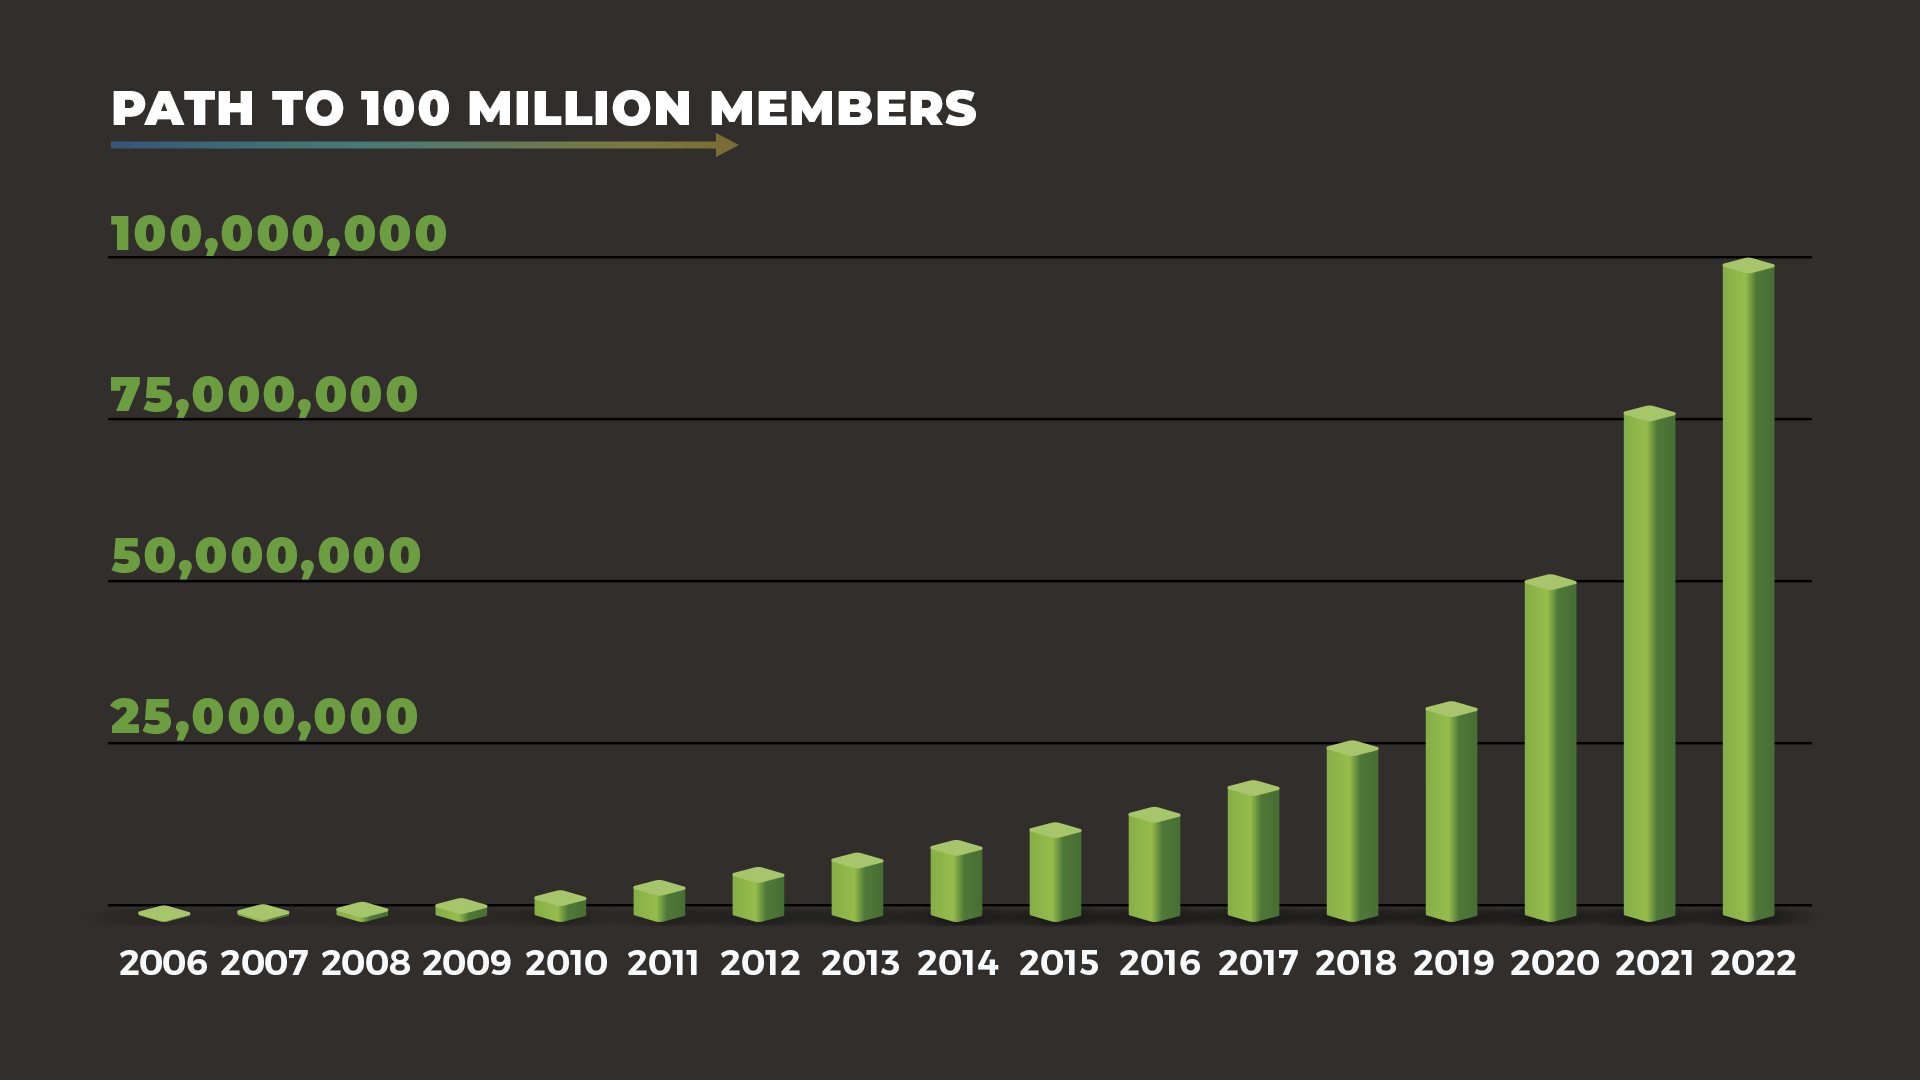
\includegraphics[scale=0.2]{images/chess.com_users.png}
    \caption{Chess.com Spielerzahlen Stand 2022}
\end{figure}

Darüber hinaus hat das Aufkommen von Live-Streaming-Plattformen wie Twitch die Art und Weise, wie Schach als Zuschauer konsumiert wird revolutioniert. 
Bekannte Spieler aus der Szene, aber auch Streamer aus anderen Sektoren zeigen hier ihre Spiele und veranstalten Turniere. 
Weitere Faktoren für den aktuellen Erfolg des Spiels ist die Netflix Serie Queens Gambit aus dem Jahr 2020, die den Weg eines Mädchens zu einer 
Profispielerin zeigt, sowie der Lockdown im selben Jahr.

\section{Motivation}
Durch die zunehmende Begeisterung für das Spielen am Computer rückt das Spiel am Brett immer mehr in den Hintergrund. 
Eine Möglichkeit die Vorteile des online Schachs und die des Brettspiels zu kombinieren ist ein DGT Smart Board. Es wird über Bluetooth 
oder USB mit dem Computer verbunden und ermöglicht dem Spieler die Züge auf einem Brett zu spielen. 
Anschließend werden die Züge an den Computer übertragen. Diese speziellen Bretter sind durch ihren hohen Preis jedoch nicht sehr attraktiv für die meisten Spieler. 
Die Idee dieser Smartboards legt die Grundlage dieses Projektes aus, welches eine Kombination aus einem realen Schachbrett und dem Computer bildet.

\section{Zielsetzung dieser Arbeit}
Ziel dieser Arbeit ist es eine Python Applikation zu entwickeln, mit welcher der Nutzer gegen einen Computer Schach spielen kann. 
Dabei soll es dem Spieler möglich sein, seine Züge auf einem realen Schachbrett zu spielen. Die gespielten Züge werden dann 
mithilfe einer Kamera an die Applikation übertragen. Somit kann Kostengünstig das Erlebnis des Online Schachs mit dem Gefühl des 
Brettspiels kombiniert werden.

Für die Implementierung der Regeln des Spiels werden keine bestehenden Bibliotheken benutzt. Der Schachcomputer soll entweder selber entwickelt werden,
oder es soll ein bestehender Computer genutzt werden.

\pagebreak
\section{Forschungsschwerpunkte}
Um die Zielsetzung zu erreichen, soll diese Arbeit folgende Aspekte behandeln:

\begin{enumerate}
    \item Digitale Bildverarbeitung
    \item Algorithmen für Schachcomputer
    \item Objektorientierte Programmierung in Python
\end{enumerate}
 
\section{Struktur}
Kapitel 2 befasst sich mit den Feinheiten der digitalen Bildverarbeitung, einem wichtigen technologischen Aspekt, 
der bei der Entwicklung des Schachsystems genutzt wurde. Dieser Abschnitt umfasst Unterpunkte zu Bildgrundlagen, Vorverarbeitung, Farbfilterung, 
Formerkennung, Segmentierung, Transformation und Merkmalsextraktion.

Danach kommt eine Einführung in die Grundlagen der Architektur und Funktionalität von Schachcomputern.
Es wird aufgezeigt welche Algorithmen in diesen Computern verwendet werden und welche verschiedenen Ansätze es gibt.
Vor allem wird zwischen Computern mit und ohne maschinellen Lernen unterschieden.

Kapitel 4 diskutiert Überlegungen zur Benutzeroberfläche und zur Programmiersprache. Hier wird die Wahl der Programmiersprache gerechtfertigt, 
in der Entwicklung verwendete Bibliotheken werden aufgezeigt und das Design von Benutzeroberflächen sowie Überlegungen zur Benutzererfahrung werden untersucht. 

Im Anschluss wird die Erstellung der Anwendung erklärt. Das Design und die Architektur des Systems werden erläutert und der Spielverlauf sowie 
die Herausforderungen während des Entwicklungsprozesses werden aufgezeigt.

Das letzte Kapitel enthält das Fazit und die zukünftigen Aussichten. Hier werden die wichtigsten Ergebnisse aus der Arbeit 
zusammengefasst und ein Ausblick auf potenzielle zukünftige Arbeiten und Verbesserungen gegeben.
	%!TEX root = ../dokumentation.tex

\chapter{Einführung in die digitale Bildverarbeitung}
Die digitale Bildverarbeitung ist ein wesentlicher Aspekt der Informatik, welcher sich stetig weiterentwickelt.
Sie ermöglicht visuelle Daten zu interpretieren und die wertvollen Informationen daraus zu extrahieren. 

Die Wurzeln der Bildverarbeitung reichen bis in die 1960er Jahre zurück, als Computer aufkamen, die leistungsstark genug waren, 
um die Rechenanforderungen von Bilddaten zu bewältigen. Ihre Ursprünge findet sie in der Raumfahrtindustrie, wo es zur Verbesserung der
Qualität von Mondbildern Verwendung fand.~\cite{Brian_2017_spacefoundation}

Das Potenzial der Bildverarbeitung wurde jedoch schnell erkannt und fand schnell auch in anderen Bereichen eine Anwendung.
Im digitalen Zeitalter spielt sie eine Rolle in Bereichen wie der medizinischen Bildgebung über autonome Fahrzeuge, Überwachung und vielen mehr.
Das Wesen der Bildverarbeitung liegt in der Übersetzung einer visuellen Eingabe in eine mathematische Darstellung, welche von Computern verstanden werden kann.
Durch diese Umwandlung können Computer sie analysieren und manipulieren.~\cite{Kernel_2023_wikipedia}
Die folgenden Kapitel beschäftigen sich mit den Feinheiten der Bildverarbeitung.  

\section{Bildgrundlagen}

\subsection{Verständnis von Pixeln}
Pixel beschreiben die kleinste Einheit eines digitalen Bildes und sind somit essenziell für das Verständnis der Bildverarbeitung.
Jeder dieser Pixel beschreibt dabei einen einzelnen Punkt im Bild und hat einen bestimmten Pixelwert, welcher die Helligkeit oder Farbe 
widerspiegelt. In farbigen Bildern werden diese Pixel durch Tripletts von Farbwerten repräsentiert. Oftmals wird hierbei der RGB-Farbraum 
verwendet. RGB steht hierbei für die drei Farben des Tripletts: Rot, Grün, Blau.~\cite{J.F._Blinn_2005_ieee}

\subsection{Bildrepräsentation}
Ein digitales Bild lässt sich als zweidimensionale Funktion \(f(x,y)\) darstellen, bei der \(x\) und \(y\) die räumliche Koordinaten sind
und die Amplitude von \(f\) zu jedem Paar \((x,y)\) die Intensität oder den Grauwert des Bildes an dem Punkt repräsentieren.
Bei farbigen Bildern besteht jedes Pixel aus einer Kombination von Primärfarben. In den meisten Fällen werden diese als RGB dargestellt. 
Die Digitalisierung von Bildern ermöglicht die Anwendung verschiedener Operationen, um es zu manipulieren oder zu analysieren. 

\subsection{Farbräume}
Farbräume sind mathematische Modelle zur Darstellung von Farben. Ihr Ziel ist es Farben so zu beschreiben, dass sie für das menschliche Auge
sinnvoll sind.

\subsubsection{RGB-Farbraum}
Der am weitesten verbreitete Farbraum ist der RGB-Farbraum. Hierbei werden die Primärfarben Rot, Grün und Blau in verschiedenen
Intensitäten gemischt, um möglichst viele Farben darzustellen. Jede Farbe wird somit durch ein Triplett von Werten dargestellt.
Jeder dieser Werte beschreibt dabei die Intensität der jeweiligen Primärfarbe. Beispielsweise entspricht ein Triplett
\((0,0,0)\) Schwarz, da keine Farbe vorhanden ist, während \((255,0,0)\) Rot entspricht.
Im digitalen Kontext ist der RGB-Farbraum besonders dominant, da er für die Farbdarstellung auf Bildschirmen zuständig ist.
Die einzelnen Pixel auf dem Bildschirm emittieren Licht in den Grundfarben und der Nutzer nimmt den Pixel als die additive Mischung dieser 
Farben auf.~\cite{Vladimir_Chernov_2023_sciencedirect}

\subsubsection{HSV-Farbraum}
Ein weiterer verbreiteter Farbraum ist HSV (Hue, Saturation, Value), welcher oftmals intuitiver als der 
RGB-Farbraum ist.
\begin{figure}[ht]
    \centering
    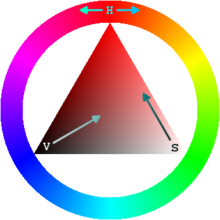
\includegraphics[scale=0.6]{images/HSV.png}
    \caption{HSV Farbraum Palette}
\end{figure}
\begin{itemize}
    \item Hue (Farbton): Der Farbton wird auf einer kreisförmigen Skala dargestellt. 
    0 oder 360 entspricht Rot, 120 Grün und 240 Blau. Die Zwischenwerte sind Mischungen der Farben.
    \item Saturation (Sättigung): Die Sättigung gibt die Intensität der Farbe an. 
    Eine Sättigung von 0 entspricht weiß, während eine Sättigung von 100 eine reine Farbe darstellt.
    Somit erscheinen Farben mit geringen Sättigungen als blass und Farben mit hoher Sättigung als voll.
    \item Value (Helligkeit): Dieser Wert spiegelt die Helligkeit oder Intensität des Lichts wider, welches von der Farbe ausgeht.
    Ein Wert von 0 stellt also Schwarz dar, während ein Wert von 100 eine Farbe in voller Helligkeit darstellt.
\end{itemize}
Der HSV-Farbraum findet vor allem Anwendung in Aufgaben, bei denen eine intuitive Steuerung wichtig ist. Beispielsweise das Ausfiltern einer Farbe durch den Nutzer.~\cite{Vladimir_Chernov_2023_sciencedirect}
\subsubsection{Graustufen}
Grayscale, oder Graustufen bezeichnen eine Darstellung von Bildern, bei welcher der Wert jedes Pixels die Intensität der Information wiedergibt.
In einem Graustufenbild kann jeder Pixel als ein unterschiedlicher Grauton angesehen werden, der von Schwarz (minimale Intensität) 
bis Weiß (maximale Intensität) reicht. Die verschiedenen Töne zwischen diesen Extremen entsprechen dann den Intensitätstufen des Lichts.
Graustufenbilder werden oft bei Aufgaben verwendet, bei denen die Farbinformationen nicht notwendig sind und ablenken können. 
Beispielsweise werden Graustufenbilder verwendet, wenn der Computer eine bestimmte Form in einem Bild finden soll, da 
Bildverarbeitungstechniken wie die Kanten-Erkennung mit Intensitätsinformationen arbeiten.
Die Verwendung von Graustufen kann außerdem die Rechenkomplexität verringern und somit die Leistung verbessern.

Im Kontext der Farbraum Umwandlung kann ein RGB-Bild oft in Graustufen umgewandelt werden, indem ein gewichtetes Mittel der RGB-Werte genommen wird. 
Diese Gewichte berücksichtigen die menschliche Wahrnehmung, da das menschliche Auge empfindlicher auf Grün und weniger empfindlich auf Blau reagiert.
Die typische Formel zur Umwandlung von RGB in grayscale ist \(grayscale = 0,299*R + 0,587*G + 0,114*B\).~\cite{Dr._Daniel_Slieter_2023_dhbw-stuttgart}

\section{Bildvorverarbeitung}
Die Bildvorverarbeitung stellt eine kritische Stufe in der Bildverarbeitung dar. Ihre Hauptaufgabe besteht darin, 
die Qualität und Lesbarkeit eines Bildes zu verbessern und das Fehlerpotenzial für nachfolgende Dateninterpretationen zu reduzieren.

\subsection{Rauschunterdrückung}
Rauschen ist in der Physik allgegenwärtig und bezeichnet eine Übertragung eines Signals mit einem ungewollten Störsignal.
Meistens handelt es sich beim Rauschen um einen stochastischen Prozess, was dazu führt, dass die verschiedenen Arten des Rauschens sich mit
ihren jeweiligen Wahrscheinlichkeitsverteilungen modellieren lassen.
Das Rauschen kann verschiedene Formen annehmen, wie zum Beispiel das additive / multiplikative Gauß'sches Rauschen, ungleich verteiltes Rauschen
und Salt-and-Pepper-Rauschen. 

\begin{figure}[ht]
    \centering
    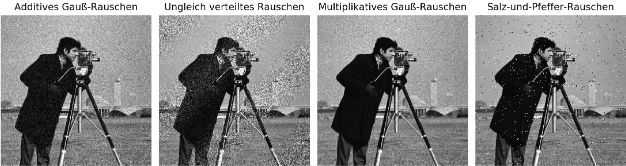
\includegraphics[scale=0.8]{images/noise.png}
    \caption{Verschiedene Arten des Rauschens}
\end{figure}

Rauschunterdrückungsalgorithmen zielen darauf ab, die Auswirkungen dieser Verzerrungen zu minimieren und die Bildqualität zu verbessern.
Je nach Art des Rauschens werden verschiedene Algorithmen benutzt.~\cite{Hannes_Bonasch_2023}

\subsection{Bildverbesserung}
Bildverbesserungstechniken werden verwendet, um visuell aufschlussreichere Bilder zu generieren, 
sowie eine Vereinfachung der nachfolgenden Signalverarbeitung und der automatischen Bildauswertung zu schaffen. Ein Beispiel für die 
Bildverbesserung ist die Bildverschärfung. Details von Bildern hängen mit einer höheren räumlichen Frequenz zusammen. Wenn diese Frequenz 
verstärkt wird, erscheint das Bild scharfer. Jedoch kann die Verschärfung auch zu weiteren Störungen führen und es muss darauf geachtet werden,
dass der durchschnittliche Bildwert konstant bleibt.~\cite{Jürgen_Beyerer_Fernando_Puente_León_Christian_Frese__2023_springer}

\subsection{Farbraum Umwandlung}
Da verschiedene Farbräume verschiedene Informationen über ein Bild liefern, kann die Umwandlung eines Bildes von einem Farbraum in einen anderen 
vorteilhaft sein. Beispielsweise wird der RGB-Farbraum oft für die Bilddarstellung verwendet während der HSV-Farbraum für die farbbasierte Bildsegmentierung
effektiver ist. Ebenso kann die Umwandlung in ein grayscale Bild die Daten vereinfachen und ist somit vorteilhaft für Aufgaben, bei denen die Farbinformationen
unnötig sind.~\cite{Noor_A._Ibraheem_2012_psu}

\section{Farbfilterung}
Die Farbfilterung gehört zu den wichtigsten Komponenten der digitalen Bildverarbeitung. Sie ist entscheidend für eine Vielzahl von Anwendungen,
wie der Objekterkennung, Gesichtserkennung und Merkmalsextraktion.

Die Farbfilterung beschäftigt sich in erster Linie mit der Trennung oder Hervorhebung bestimmter Farbbereiche in einem Bild. Dieser Prozess wird hauptsächlich durch
die Definition eines bestimmten Farbbereichs oder mehrerer Farbbereiche im Farbraum eines Bildes erleichtert. Anschließend werden Pixel, die innerhalb 
dieser festgelegten Bereiche fallen, beibehalten, während die anderen in der Regel auf Schwarz gesetzt werden, 
wodurch die gewünschten Farbkomponenten effektiv isoliert werden. Es gibt verschiedene Farbfilterungen, je nach Farbbereich. 
Die populärsten sind jedoch HSV-Farbfilterung und Graufilterung. Der Grund für die Nutzung des HSV-Filters statt eines RGB-Filters 
ist die Entkopplung der Farb- und Helligkeitsinformationen. Der Filter wird in Aufgaben verwendet, bei denen die Robustheit gegenüber 
Beleuchtungsänderungen relevant ist. 

\section{Formerkennung}
Neben der Farbfilterung ist die Formerkennung eine grundlegende Rolle in der Bildverarbeitung und unverzichtbar in einer Vielzahl von Anwendungen,
die von Objekterkennung und Objektverfolgung über medizinische Bildgebung bis hin zur maschinellen Bildverarbeitung reichen. Im Folgenden wird 
die Mechanik der Formerkennung erläutert und verwendete Methoden aufgezeigt.

\subsection{Kanten-Erkennungsmethoden}
Die Kanten-Erkennung ist einer der Schlüsselschritte in der Formerkennung. In erster Linie befasst sie sich mit der Identifizierung von Punkten in einem Bild,
an denen die Helligkeit stark wechselt, beziehungsweise Punkte an denen der Gradient der  Bildintensitätsfunktion hoch ist. Für diesen Zweck wurden diverse
Methoden entwickelt. Die bekanntesten sind die Sobel- und Canny-Operatoren. Die Operatoren unterscheiden sich dabei in ihren Ansätzen und 
liefern unterschiedliche Ergebnisse, abhängig von den spezifischen Anforderungen der Anwendung.~\cite{AHMED_SHIHAB_AHMED_2018_jatit}

\subsubsection{Sobel-Operator}
Der Sobel-Operator wird verwendet,  um die Gradienten der Bildintensität an jedem Pixel zu bestimmen und 
um Regionen zu markieren, falls deutliche Intensitätskontraste auftreten. Er läuft durch das Bild mit einem Paar von 3$\times$3-Kerneln, 
die auf senkrecht und waagrecht zur Pixelmatrix verlaufende Kanten reagieren. Beispielhafte Kernel könnten wie folgt aussehen:

\begin{figure}[h!]
\centering
\begin{align*}
    A &= \begin{bmatrix}
        -1 & 0 & 1 \\
        -2 & 0 & 2 \\
        -1 & 0 & 1
    \end{bmatrix},
    & B &= \begin{bmatrix}
        -1 & -2 & -1 \\
        0 & 0 & 0 \\
        1 & 2 & 1
    \end{bmatrix}
\end{align*}
\caption{(A) Sobel vertikal-Operator (B) Sobel horizontal-Operator}
\end{figure}

Die resultierenden Kanten werden als Grauwertbilder dargestellt, 
bei denen Kanten auf einem schwarzen Hintergrund zu sehen sind. Die Ausgabe kann anschließend binarisiert werden, 
um Kanten klar vom Rest des Bildes zu trennen und für weitere Bildverarbeitungsaufgaben verwendet werden.~\cite{AHMED_SHIHAB_AHMED_2018_jatit}

\subsubsection{Canny-Operator}
Im Gegensatz dazu verwendet der Canny-Operator eine Reihe von Schritten, um präzisere und weniger störanfällige Kanteninformationen zu erzeugen.
Er beginnt mit der Glättung des Bildes durch eine Gaußsche Glättung, um das Rauschen zu reduzieren. Anschließend wird ein Schritt durchgeführt, 
welcher dem Sobel-Operator ähnelt, um die Gradientenmagnituden und -richtungen zu bestimmen. Die Kanten werden nun durch eine Nicht-Maximum-Unterdrückung
geschärft. Im letzten Schritt wird die Schwellenwertbildung mit Hysterese angewendet, um sicherzustellen, dass nur die stärksten Kanten im Resultat 
zu sehen sind.

Die Wahl zwischen den Operatoren hängt stark vom Anwendungsfall ab. Die Implementation des Sobel-Operators ist einfacher, jedoch ist er anfälliger 
für Bildrauschen und kann bei feinen Kanten ungenau sein. Der Canny-Operator ist dem Sobel-Operator damit in der Qualität der Ergebnisse überlegen,
jedoch steigt durch die erhöhte Komplexität auch die Anforderungen an die Rechenleistung und den benötigten Speicher.~\cite{AHMED_SHIHAB_AHMED_2018_jatit}

\subsection{Konturerkennung}
Konturen sind ein weiteres wichtiges Merkmal in der Bildverarbeitung, um einen Rückschluss auf Objekte zu geben. Die Erkennung beinhaltet das 
Gruppieren von Kantenpixeln zu zusammenhängenden Kurven. Konturerkennungstechniken bieten somit eine Möglichkeit zur Erkennung und Visualisierung
von Objektgrenzen und liefern eine ganzheitliche Darstellung der Form im Vergleich zu den isolierten Kantenpixeln.~\cite{Xin-Yi_Gong_2018_springer}

\subsection{Formerkennung}
Nach der Erkennung von Kanten und Konturen besteht der nächste Schritt in der Erkennung von Formen. Das geschieht durch den
Vergleich der erkannten Form mit einem Satz bekannter Formen. Dieser Prozess kann einfache geometrische Formen (Kreise, Quadrate, etc.) 
oder komplexere Formen beinhalten, sofern diese erlernt wurden. Die Formerkennung geht oft Hand in Hand mit einem Ansatz des maschinellen Lernens
und Mustererkennungsalgorithmen, um die Formen zu klassifizieren.~\cite{Sambarta_Dasgupta_2009_springer}

\section{Bildsegmentierung}
Die Bildsegmentierung ist entscheidend für die Extraktion spezifischer Merkmale oder Objekte in einem Bild. Im Wesentlichen transformiert sie ein
Bild in eine Ansammlung von Regionen mit identifizierbaren Eigenschaften. Diese Transformation liefert eine Darstellung des Bildes, die topologische
und geometrische Informationen liefert und als Grundlage für die weitere Bildanalyse und Interpretation dient.

\subsection{Techniken zur Bildsegmentierung}
Je nach Anwendungsfall gibt es verschiedene Techniken zur Bildsegmentierung.

\subsubsection{Schwellenwertsetzung}
Die Schwellenwertsetzung ist wegen ihrer Einfachheit weit verbreitet. Ihr Ziel ist es, den Vordergrund eines Bildes vom Hintergrund zu trennen, 
indem ein Graustufen- oder Farbbild in ein Binärbild umgewandelt wird.

\begin{figure}[h]
    \centering
    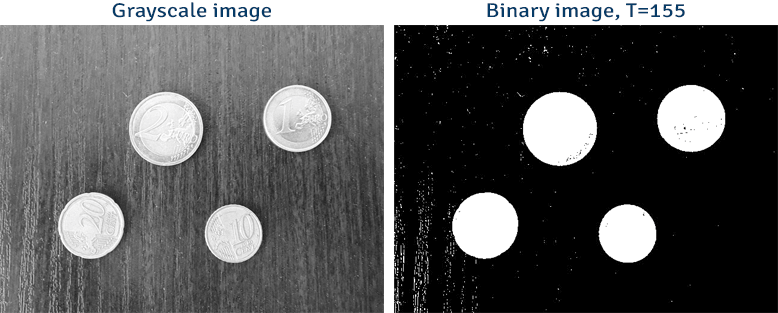
\includegraphics[scale=0.5]{images/threshholding.png}
    \caption{Schwellenwertsetzung Beispiel}
\end{figure}

Wie in Abbildung 3.4 zu sehen ist, wird ein zunächst ein Schwellwert gewählt. Je kleiner dieser ist, desto kleinere Objekte werden erkannt.
Anschließend werden alle Pixelintensitätswerte über oder unter diesem Schwellwert auf einen bestimmten Wert gesetzt, um die gewünschte Segmentierung
zu erreichen. Ein Vorteil der Schwellenwertsetzung ist die einfache Implementation, jedoch kann es bei variablen Lichtverhältnissen zu fehlerhaften
Ergebnissen kommen. 

\subsubsection{Clustering}
Eine andere Gruppe von Techniken zur Bildsegmentierung umfasst das Clustering. Ein Beispiel für diese Technik ist K-means, 
welcher die Pixel mit ähnlichen Attributen zusammenfasst. Der K-means-Algorithmus segmentiert dabei ein Bild in K Cluster, 
wobei jedem Pixel das Cluster mit dem nächstgelegenen mittleren Intensitätswert oder Farbvektor zugeordnet wird. 
Trotz der Vielseitigkeit dieses Algorithmus, reagieren die Ergebnisse sehr empfindlich auf die Parameter Auswahl und der Algorithmus ist
sehr rechenintensiv.~\cite{G.B._Coleman_1979_ieee}

\section{Bildtransformation}
Bildtransformationen sind Operationen in der Bildverarbeitung, die Bilder zur Analyse, Interpretation oder Visualisierung modifizieren. 
Diese Operationen lassen sich in räumliche Transformationen, die die räumlichen Attribute des Bildes verändern, 
und Frequenzbereich-Transformationen, die den Frequenzinhalt des Bildes manipulieren, unterteilen.

\subsection{Räumliche Transformationen}
Räumliche Transformationen sind Bildoperationen, die die Position und Ausrichtung der Pixel in einem Bild ändern 
und dabei ihre Nachbarschaftsbeziehungen beibehalten.

\subsubsection{Skalierung}
Die Skalierung ist eine Transformation, die die Größe eines Bildes ändert. Sie kann sowohl eine Vergrößerung als auch eine Verkleinerung sein, 
beide verändern die Breite und Höhe des Bildes. Dabei ist es entscheidend, das Seitenverhältnis während der Skalierung beizubehalten, 
um eine Verzerrung des Bildes zu verhindern.

\subsubsection{Rotation}
Die Rotation ist eine Transformation, die die Ausrichtung eines Bildes ändert. 
Sie beinhaltet das Drehen der Pixel des Bildes um einen bestimmten Punkt, typischerweise das Bildzentrum, um einen bestimmten Winkel. 
Wie andere räumliche Transformationen muss darauf geachtet werden, Pixelinterpolation zu vermeiden und die Bildqualität zu erhalten.
Die Pixelinterpolation beschreibt dabei das Problem, dass die ursprünglichen Pixel nicht in das Pixelgitter des neuen Bildes passen.
Dann muss eine Entscheidung getroffen werden, welcher Wert dem neuen Pixel zugeordnet wird.~\cite{Don_Lancaster_2007_ollintec}

\subsubsection{Translation}
Die Translation ist eine räumliche Transformation, die ein Bild in x- und/oder y-Richtung verschiebt. 
Dabei wird jeder Pixel an einen neuen Ort verschoben, ohne seinen Wert zu ändern.

\subsection{Transformationen im Frequenzbereich}
Transformationen im Frequenzbereich beinhalten die Umwandlung eines Bildes vom Raum- in den Frequenzbereich, 
bei dem die Informationen des Bildes in Bezug auf ihren Frequenzinhalt dargestellt werden.
Der Frequenzinhalt eines Bildes bezieht sich auf die Rate, mit der die Pixelintensitäten (oder Farben) im Bild ändern. 
Diese Änderungsrate wird in Form von Frequenzen gemessen.

\subsubsection{Fourier-Transformation}
Die Fourier-Transformation ist ein Standardwerkzeug zur Analyse des Frequenzinhalts eines Bildes. 
Sie zerlegt ein Bild in seine Sinus- und Kosinus-Komponenten und zeigt die periodischen Strukturen des Bildes und ihre Ausrichtungen auf. 
Die resultierende Darstellung ist komplex und enthält sowohl Amplituden- als auch Phaseninformationen, die beide notwendig sind, 
um das Originalbild vollständig zu rekonstruieren.~\cite{S._Sridhar_2014_mecs-press}

\subsubsection{Wavelet-Transformation}
Eine weitere Technik zur Frequenzbereichsanalyse ist die Wavelet-Transformation. Im Gegensatz zur Fourier-Transformation, 
welche das Bild global betrachtet, verwendet die Wavelet-Transformation Wavelets, um das Bild lokal zu analysieren 
und eine Zeit-Frequenz-Darstellung zu liefern. Diese Eigenschaft ist nützlich für die Analyse von Bildern mit 
nicht-stationären Signalen oder mit Strukturen auf mehreren Skalen.~\cite{S._Sridhar_2014_mecs-press}

\subsection{Anwendungen von Bildtransformationen}
Bildtransformationen spielen eine entscheidende Rolle in verschiedenen Anwendungen. Räumliche Transformationen werden in der Bildregistrierung verwendet, 
bei der Bilder zum Vergleich ausgerichtet werden, und in der Datenvergrößerung für maschinelles Lernen, bei der Bildvarianten erstellt werden, 
um Trainingsdaten zu erweitern. 
Transformationen im Frequenzbereich hingegen werden in der Bildfilterung, Kompression und Rauschreduzierung verwendet.
Zum Beispiel wird die Fourier-Transformation in der MRT-Bildgebung eingesetzt. Die Wavelet-Transformation wird in der JPEG2000-Kompression verwendet, welche 
einen verbesserten Nachfolger des JPEG-Standards darstellt.
Durch diese Anwendungen tragen Bildtransformationen erheblich zur Fähigkeit bei, visuelle Daten zu analysieren, zu interpretieren und zu nutzen.~\cite{H._Burkhardt_uni-freiburg}

\section{Merkmalsextraktion}
Die Merkmalsextraktion besteht darin, relevante Informationen aus einem Bild zu extrahieren. Dieser Prozess ermöglicht eine Reduzierung 
der Datenmenge bei gleichzeitiger Beibehaltung der wesentlichen Details, wodurch Aufgaben wie Bilderkennung, 
Objekterkennung oder das Training von maschinellem Lernen erleichtert werden.

Merkmale können als messbare Eigenschaften beobachteter Auffälligkeiten definiert werden. Im Fall von Bildern entsprechen diese Merkmale 
oft ausgeprägten Elementen der Bildstruktur, wie Kanten, Ecken oder Bereiche mit einer bestimmten Textur oder Farbe. 
Ziel der Merkmalsextraktion ist es, das Bild so zu repräsentieren, dass die Beschreibung vereinfacht oder das Potenzial 
für nachfolgende Analysen oder Klassifikationen verbessert wird.~\cite{Shambhavi_Jain_2017_ieee}

\subsection{Techniken zur Merkmalsextraktion}
Es gibt diverse Techniken, welche zur Extraktion von Merkmalen aus Bildern verwendet werden können. 
Zwei populäre Techniken, die häufig im Bereich der Bildverarbeitung und Computer Vision verwendet werden, 
sind das \ac{SIFT} und das \ac{SURF}.~\cite{Shambhavi_Jain_2017_ieee}

\subsubsection{SIFT}
\ac{SIFT} ist eine Methode zur Erkennung und Beschreibung lokaler Merkmale in Bildern. 
Die mit dieser Methode extrahierten Merkmale sind immun gegenüber Bildskalierungen und -rotationen 
und zeigen eine robuste Übereinstimmung über einen erheblichen Bereich von Verzerrungen, Änderungen des 3D-Blickpunkts, 
Hinzufügen von Rauschen und Änderungen der Beleuchtung.~\cite{Shambhavi_Jain_2017_ieee}

\subsubsection{SURF}
\ac{SURF} ist ein weiterer Bild-Deskriptor. Es ähnelt \ac{SIFT} in vielen Aspekten, ist aber schneller und robuster gegenüber Bildtransformationen, 
was es für Echtzeitanwendungen geeignet macht und perfekt für Aufgaben ist, die eine schnelle Merkmalsextraktion erfordern.~\cite{Shambhavi_Jain_2017_ieee}
    %!TEX root = ../dokumentation.tex

\chapter{Die Architektur und Funktionalität von Schachcomputern}

\section{Einleitung}

\subsection{Die Entwicklung von Schachcomputern}
Die Geschichte der Schachcomputer zeigt die Entwicklung von künstlicher Intelligenz und Rechenleistung. 
In den 1940er Jahren wurden einige der frühesten theoretischen Arbeiten zu Schachspielcomputern von Informatikern 
wie Claude Shannon und Alan Turing unternommen. Trotz der begrenzten Rechenressourcen, die ihnen zur Verfügung standen, 
erkannten sie das Potenzial von Computern, sich in einem Spiel wie Schach zu behaupten.~\cite{History_of_chess_engines_2023_wikipedia}

Die ersten tatsächlichen Schachspielcomputer wurden jedoch erst in den 1960er und 1970er Jahren geschaffen. Diese Maschinen, 
wie das Schachspielcomputersystem von IBM namens Deep Blue, konnten auf dem Niveau eines kompetenten Menschen spielen, 
waren aber weit entfernt von der Weltklasse.

Erst mit dem Aufkommen leistungsstarker Computer und besseren Algorithmen im späten 20. und frühen 21. Jahrhundert 
waren Computer in der Lage, mit menschlichen Weltmeistern zu konkurrieren und diese zu schlagen. 
1997 machte IBMs Deep Blue weltweit Schlagzeilen, als es den amtierenden Schachweltmeister Garry Kasparow in einem Sechsspiel-Match besiegte.~\cite{Chris_Higgins_2017_mentalfloss}


Seitdem hat die Leistungsfähigkeit von Schachcomputern nur noch zugenommen, wobei Programme wie Stockfish und Komodo selbst die stärksten 
menschlichen Spieler übertreffen. Und in den letzten Jahren wurde Aufstieg des maschinellen Lernens im Schach gesehen, 
wobei das AlphaZero-Programm von Google sich selbst trainiert, um in nur wenigen Spielstunden ein Weltklassespieler zu werden.~\cite{History_of_chess_engines_2023_wikipedia}

\subsection{Rolle und Zweck von Schachcomputern}
Der Zweck von Schachcomputern geht über das einfache Gewinnen von Spielen hinaus. Auf einer grundlegenden Ebene besteht das Ziel eines Schachcomputers darin, 
menschenähnliches Denken und Entscheiden im Kontext des Spiels zu simulieren. Schachcomputer dienen daher als Plattform zur Erforschung komplexer Konzepte 
in der künstlichen Intelligenz, einschließlich Suchalgorithmen, Mustererkennung und strategischer Planung.

Darüber hinaus bieten Schachcomputer praktische Anwendungen. Sie dienen menschlichen Spielern als wertvolle Werkzeuge, indem sie hochrangige Übungsgegner 
bereitstellen und eine detaillierte Analyse von Spielen anbieten. Schachcomputer stellen ebenfalls eine Hilfe für neue Spieler dar, indem sie durch
detaillierte Analysen der Spiele die Schwächen eines Spielers individuell zu erkennen und den Nutzer darauf aufmerksam machen. 
Ein Beispiel dafür ist die Spielanalyse von Chess.com, bei der ein virtueller Coach nochmal über das Spiel mit dem Nutzer geht und ihm Tipps gibt.

Mit Blick auf die Zukunft ist es wahrscheinlich, dass Schachcomputer eine bedeutende Rolle in der weiteren Entwicklung spielen werden, 
da das Feld der künstlichen Intelligenz sich weiterhin entwickelt.~\cite{Larry_Greenemeier_2017_scientificamerican}

\section{Schachcomputer ohne maschinelles Lernen}

\subsection{Definition}
Schachcomputer ohne maschinelles Lernen, auch als traditionelle Schach-Engines bekannt und stellen eine Klasse von künstlichen Intelligenzprogrammen dar, 
die entwickelt wurden, um Schach zu spielen. Im Gegensatz zu Bots, die auf maschinellem Lernen basieren, lernen diese Engines nicht aus ihren Erfahrungen, 
sondern folgen einem vordefinierten Satz von Regeln und Algorithmen.
Sie nutzen deterministische und heuristische Methoden, um den Spielzustand zu bewerten und den optimalen Zug zu bestimmen.

Traditionelle Schachcomputer waren jahrzehntelang der Mainstream. Die erfolgreichsten Beispiele, wie Stockfish und Komodo, 
wurden durch viele Iterationen und Verbesserungen entwickelt und können auf einem Niveau weit über den menschlichen Fähigkeiten spielen.
Sie wenden dabei eine Vielzahl von Techniken an, um den Zustand des Spiels zu verarbeiten und zu analysieren.

\subsection{Positionsbewertung}
Die Positionsbewertung spielt eine entscheidende Komponente, die es Schachcomputern ermöglicht, die Stärke und das strategische Potenzial eines bestimmten 
Spielzustands einzuschätzen. Dieser Prozess beinhaltet die Analyse der Anordnung der Figuren und die Zuweisung eines numerischen Werts zu dieser 
Konfiguration auf der Grundlage einer Vielzahl von Kriterien.

\subsubsection{Materialgleichgewicht}
Die grundlegendste Bewertungsmethode besteht darin, den Gesamtwert der Figuren auf dem Brett für beide Seiten zu zählen. 
Jeder Figur wird ein bestimmter Wert zugewiesen (Dame: 9, Turm: 5, Läufer: 3, Springer: 3, Bauer: 1), 
und das Materialgleichgewicht ist die Differenz zwischen den beiden Seiten. Die Seite mit dem höheren Gesamtwert steht im Allgemeinen besser da.

\subsubsection{Aktivität der Figuren}
Aktive Figuren sind im Allgemeinen wertvoller als passive. Ein Springer beispielsweise, der sich in der Mitte des Bretts befindet, 
könnte potenziell acht verschiedene Felder angreifen oder darauf ziehen, während ein Springer in einer Ecke nur auf zwei Felder ziehen könnte. 
Eine Bewertungsfunktion würde dem zentraler gelegenen Springer einen höheren Wert geben.
Für jede Figur kann also eine Map angelegt werden, welche die favorisierten Felder höher gewichtet.

\begin{figure}[ht]
    \centering
    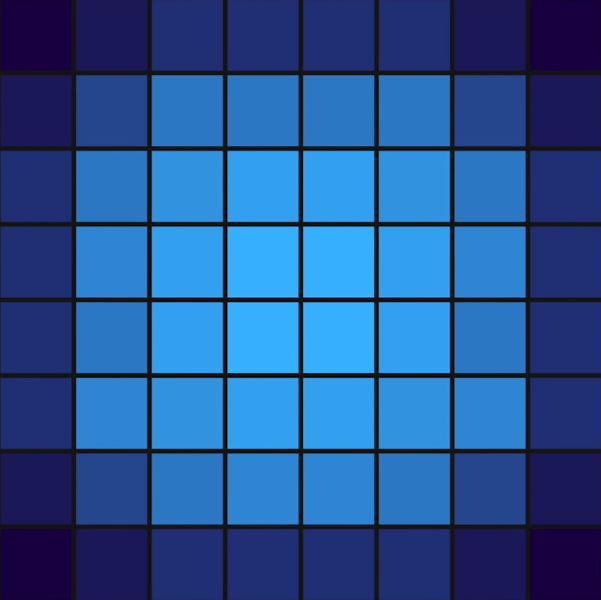
\includegraphics[scale=0.3]{images/knight_map.png}
    \caption{Springer Map}
\end{figure}

Die Abbildung 4.1 zeigt eine Beispielhafte Map für den Springer. Je heller der Blauton ist, desto höher wird das jeweilige Feld gewertet.~\cite{Lague_Sebastian_2021_youtube}

\subsubsection{Kontrolle des Zentrums}
Die Kontrolle des Zentrums ist im Allgemeinen vorteilhaft, da sie mehr Mobilität für die Figuren des Spielers 
bietet und die Position des Gegners einschränken kann.

\subsubsection{Kontrolle der Felder}
Felder, die von einem Spieler kontrolliert werden und die dieser angreift oder verteidigt, sind wertvoll, insbesondere wenn sie im Zentrum oder
im gegnerischen Spielraum liegen.

\subsubsection{Königssicherheit}
Die Sicherheit des Königs ist ein weiterer wichtiger Faktor. Ein Spieler, dessen König möglichen Schachmatt-Drohungen ausgesetzt ist, 
steht im Nachteil. Deshalb berücksichtigen Bewertungsfunktionen Faktoren wie die Frage, ob der König von Bauern geschützt ist oder
ob der Gegner viele Figuren in der Nähe des Königs hat.

\subsubsection{Bauernstruktur}
Trotz ihrer geringen Punktewertung können Bauern und ihre Struktur einen großen Einfluss auf das Spiel haben. 
Bauernketten, doppelte Bauern, isolierte Bauern, durchgebrochene Bauern sind alles wichtige Faktoren bei der Positionsbewertung. 
Im Allgemeinen werden starke Bauernstrukturen bevorzugt vor allem im weiteren Spielverlauf.

\subsection{Suchtechniken}
Suchtechniken sind das Kernstück des Entscheidungsprozesses eines Schachcomputers. Techniken wie Minimax-Suche, werden verwendet, um den Spielbaum zu erkunden, 
der die zukünftigen Möglichkeiten im Spiel repräsentiert. Die Idee besteht darin, das Worst-Case-Szenario zu minimieren, 
unter der Annahme eines optimalen Spiels des Gegners.

\begin{figure}[ht]
    \centering
    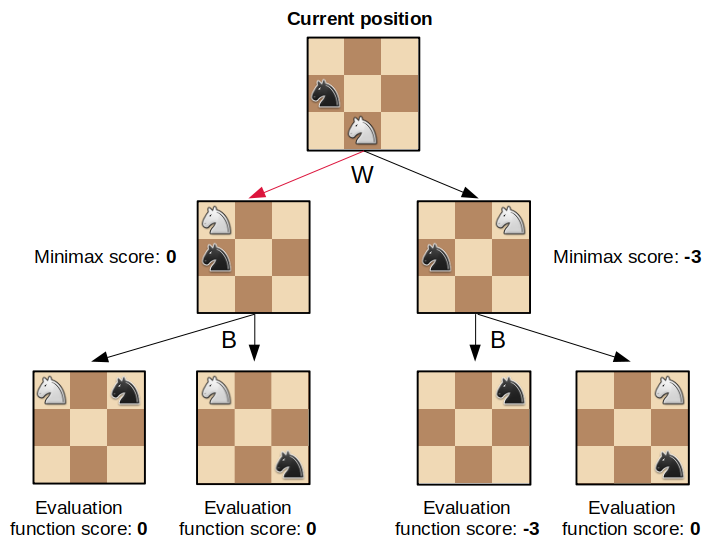
\includegraphics[scale=0.3]{images/chess_minimax_position.png}
    \caption{Minimax Algorithmus}
\end{figure}

Dabei wird der Suchbaum bis zur untersten Stufe durchgelaufen und die Endposition evaluiert. In Abbildung 4.1 ist die Evaluation für den Fall unten links
0. Diese Evaluation wird dann anschließend mit den anderen möglichen Ausgängen aus der vorherigen Position verglichen. Nun wird zwischen weißem und schwarzem 
Spieler unterschieden. Weiß stellt dabei den zu maximierenden Spieler und schwarz den zu minimierenden Spieler dar. Das heißt, dass 
der weiße Spieler eine Position mit einer möglichst hohen Evaluationszahl erlangen will und umgekehrt. Der beste Ausgang wird dann an die darüberliegende Ebene 
übertragen. Dieses Prozedere wird bis zur obersten Ebene wiederholt, sodass der Computer dann den Zug spielt, der für ihn das beste Ergebnis, unter 
Annahme des perfekten Spiels des Gegners.~\cite{Diderich2001}

\subsection{Alpha-Beta-Pruning}
Alpha-Beta-Pruning ist eine bedeutende Verbesserung des Minimax-Algorithmus, der in Entscheidungsfindung und Spieltheorie verwendet wird. 
Dieser Suchalgorithmus wird hauptsächlich in Spielen eingesetzt, in denen die Spieler abwechselnd ziehen. 
Sein Zweck ist es, die Anzahl der vom Minimax-Algorithmus ausgewerteten Knoten zu reduzieren, wodurch die Effizienz erhöht wird.

Obwohl der Minimax-Algorithmus konzeptionell einfach und effektiv ist, ist er auch rechenintensiv, insbesondere für Spiele mit großen Entscheidungsbäumen wie Schach. 
Der Algorithmus muss alle Knoten des Baumes durchlaufen, um eine Entscheidung zu treffen, was bei großen Suchräumen sehr ineffektiv ist.

Alpha-Beta-Pruning bietet eine Lösung für dieses Problem. Es handelt sich um eine Optimierungsmethode, die die Anzahl der vom Minimax-Algorithmus 
zu bewertenden Knoten erheblich reduziert. Es funktioniert, indem es Zweige im Spielbaum eliminiert, 
die nicht durchsucht werden müssen, weil bereits ein besserer Zug verfügbar ist.

Dieser Algorithmus hält für jeden Knoten im Spielbaum zwei Werte, Alpha und Beta, fest. Alpha repräsentiert die minimale Punktzahl, 
die der maximierende Spieler sicher hat, während Beta die maximale Punktzahl darstellt, die der minimierende Spieler sicher hat. 
Während der Suche, wenn der maximierende Spieler eine höhere oder gleich hohe Punktzahl (durch ein Kind des Knotens) findet als Beta, kann er aufhören, 
die anderen Kinder des Knotens zu betrachten, weil der minimierende Spieler niemals zulassen wird, dass das Spiel diesen Knoten erreicht. 
Ebenso kann der minimierende Spieler aufhören zu suchen, wenn er eine Punktzahl findet, die niedriger oder gleich Alpha ist, 
weil der maximierende Spieler niemals zulassen wird, dass das Spiel diesen Knoten erreicht.
\begin{figure}[ht]
    \centering
    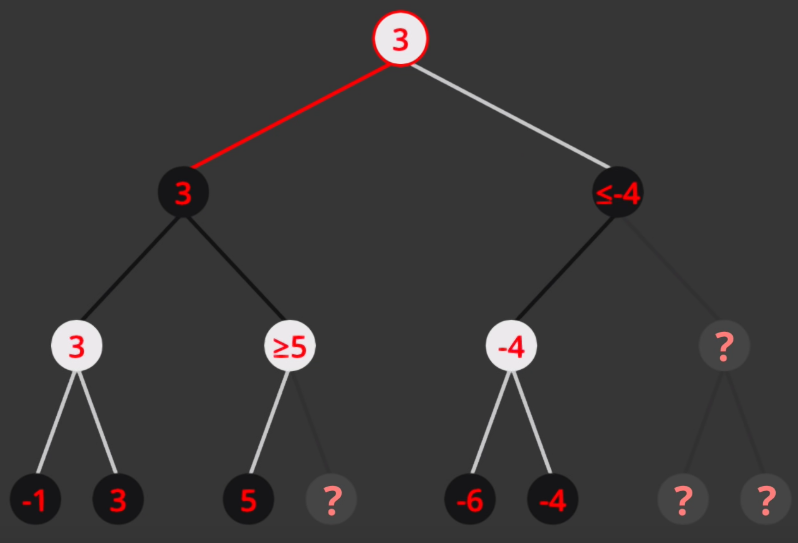
\includegraphics[scale=0.5]{images/alpha-beta-pruning.png}
    \caption{Alpha-Beta-Pruning}
\end{figure}

Auf diese Weise ermöglicht Alpha-Beta-Pruning dem Minimax-Algorithmus, mehr Knoten zu prüfen, 
die wahrscheinlich die endgültige Entscheidung beeinflussen, und Knoten zu verwerfen, die das nicht tun. 
In der Abbildung 4.2 sind die verworfenen Knotenpunkte mit Fragezeichen gekennzeichnet.
Dies macht den Suchalgorithmus weitaus effizienter und ermöglicht es ihm, tiefer in den Spielbaum vorzudringen, was wiederum die KI stärker macht.

Alpha-Beta-Pruning hat keinen Einfluss auf das endgültige Ergebnis des Minimax-Algorithmus. Der Algorithmus macht die Berechnung nur schneller. 
Er ermöglicht es, Zweige, die keinen Einfluss auf die endgültige Entscheidung haben, zu verwerfen und dadurch Rechenressourcen und Zeit zu sparen. 
Für Spiele wie Schach ist es eine notwendige Verbesserung um den Computer in Echtzeit spielen zu lassen.

Jedoch hängt die Effizienz und gesparte Zeit stark davon ab, in welcher Reihenfolge die Züge durchprobiert werden.~\cite{Aayush_Parashar_2023_springer}

\subsection{Zugsortierung}  
Das Ziel der Zugsortierung in Schach-Engines besteht darin, die Effizienz des Suchalgorithmus zu verbessern.
Durch die zuerst erfolgende Untersuchung vielversprechender Züge kann die Schach-Engine schneller einen Cut-Off in ihrem Suchbaum erreichen. 
Cut-Offs treten im Minimax-Algorithmus mit Alpha-Beta-Pruning auf, wenn die Engine feststellt, dass sie bereits einen besseren Zug gefunden hat als den, 
den sie gerade in Betracht zieht, sodass sie aufhören kann, den aktuellen Zug weiter zu analysieren.
Es wird hier zwischen verschiedenen Klassen an Zügen unterschieden.~\cite{Move_Ordering_2023_chessprogramming}

\subsubsection{Schlagzüge}
Züge, die ein gegnerisches Stück schlagen, werden in der Regel zuerst untersucht, da sie die Bewertung der 
Stellung signifikant verändern können.~\cite{Move_Ordering_2023_chessprogramming}

\subsubsection{Killerzüge}
Killerzüge sind Züge, die keine Schlagzüge sind, aber in einem Geschwisterknoten im Suchbaum auf der gleichen Tiefe einen Cut-Off verursacht haben. 
Diese Züge werden gespeichert und frühzeitig ausprobiert, wenn andere Knoten auf der gleichen Tiefe im Suchbaum analysiert werden.~\cite{Move_Ordering_2023_chessprogramming}

\subsubsection{Geschichts-Heuristik}
Diese Heuristik gibt Zügen, die in der Vergangenheit Cut-Offs verursacht haben, Priorität.
Sie basiert auf der Idee, dass, wenn ein Zug in einer Position gut war, er auch in einer anderen, aber ähnlichen Position gut sein könnte.~\cite{Move_Ordering_2023_chessprogramming}

\subsubsection{Gegen-Züge}
Der letzte Zug, der einen Cut-Off verursacht hat, wird für jedes Paar aus dem Zug des Gegners und dem eigenen Zug gespeichert.
Dies basiert auf der Idee, dass bestimmte Züge gute Antworten auf bestimmte Züge des Gegners sind.~\cite{Move_Ordering_2023_chessprogramming}

\subsubsection{Hauptvarianten-Züge}
Bei iterativen Suchen wird der beste Zug aus der vorherigen Iteration zuerst in der nächsten Iteration ausprobiert.~\cite{Move_Ordering_2023_chessprogramming}

\subsection{Transpositionstabellen}
Im Bereich des Schach-Computings spielen Transpositionstabellen eine entscheidende Rolle, um den Entscheidungsprozess des Computers effizient zu gestalten. 
Transpositionstabellen sind im Wesentlichen eine Form von Caching, die der Bot nutzt, um die Bewertung von zuvor berechneten Positionen zu speichern. 
Die gespeicherten Bewertungen können später abgerufen werden, was die Notwendigkeit einer kostenintensiven Neuberechnung vermeidet 
und die Leistung der Engine erheblich verbessert.~\cite{Jos_W._H_1970_researchgate}

\subsubsection{Verständnis der Transpositionstabellen}
Transpositionstabellen basieren auf dem Konzept der Transpositionen im Schach. 
Eine Transposition tritt auf, wenn eine bestimmte Position durch mehr als eine Zugfolge erreicht wird. 
Viele verschiedene Partien können zu der gleichen Position führen, und das Erkennen dieser identischen Positionen ist der 
Schlüssel zur Optimierung des Entscheidungsprozesses einer Chess-Engine.~\cite{Jos_W._H_1970_researchgate}

\begin{figure}[ht]
    \centering
    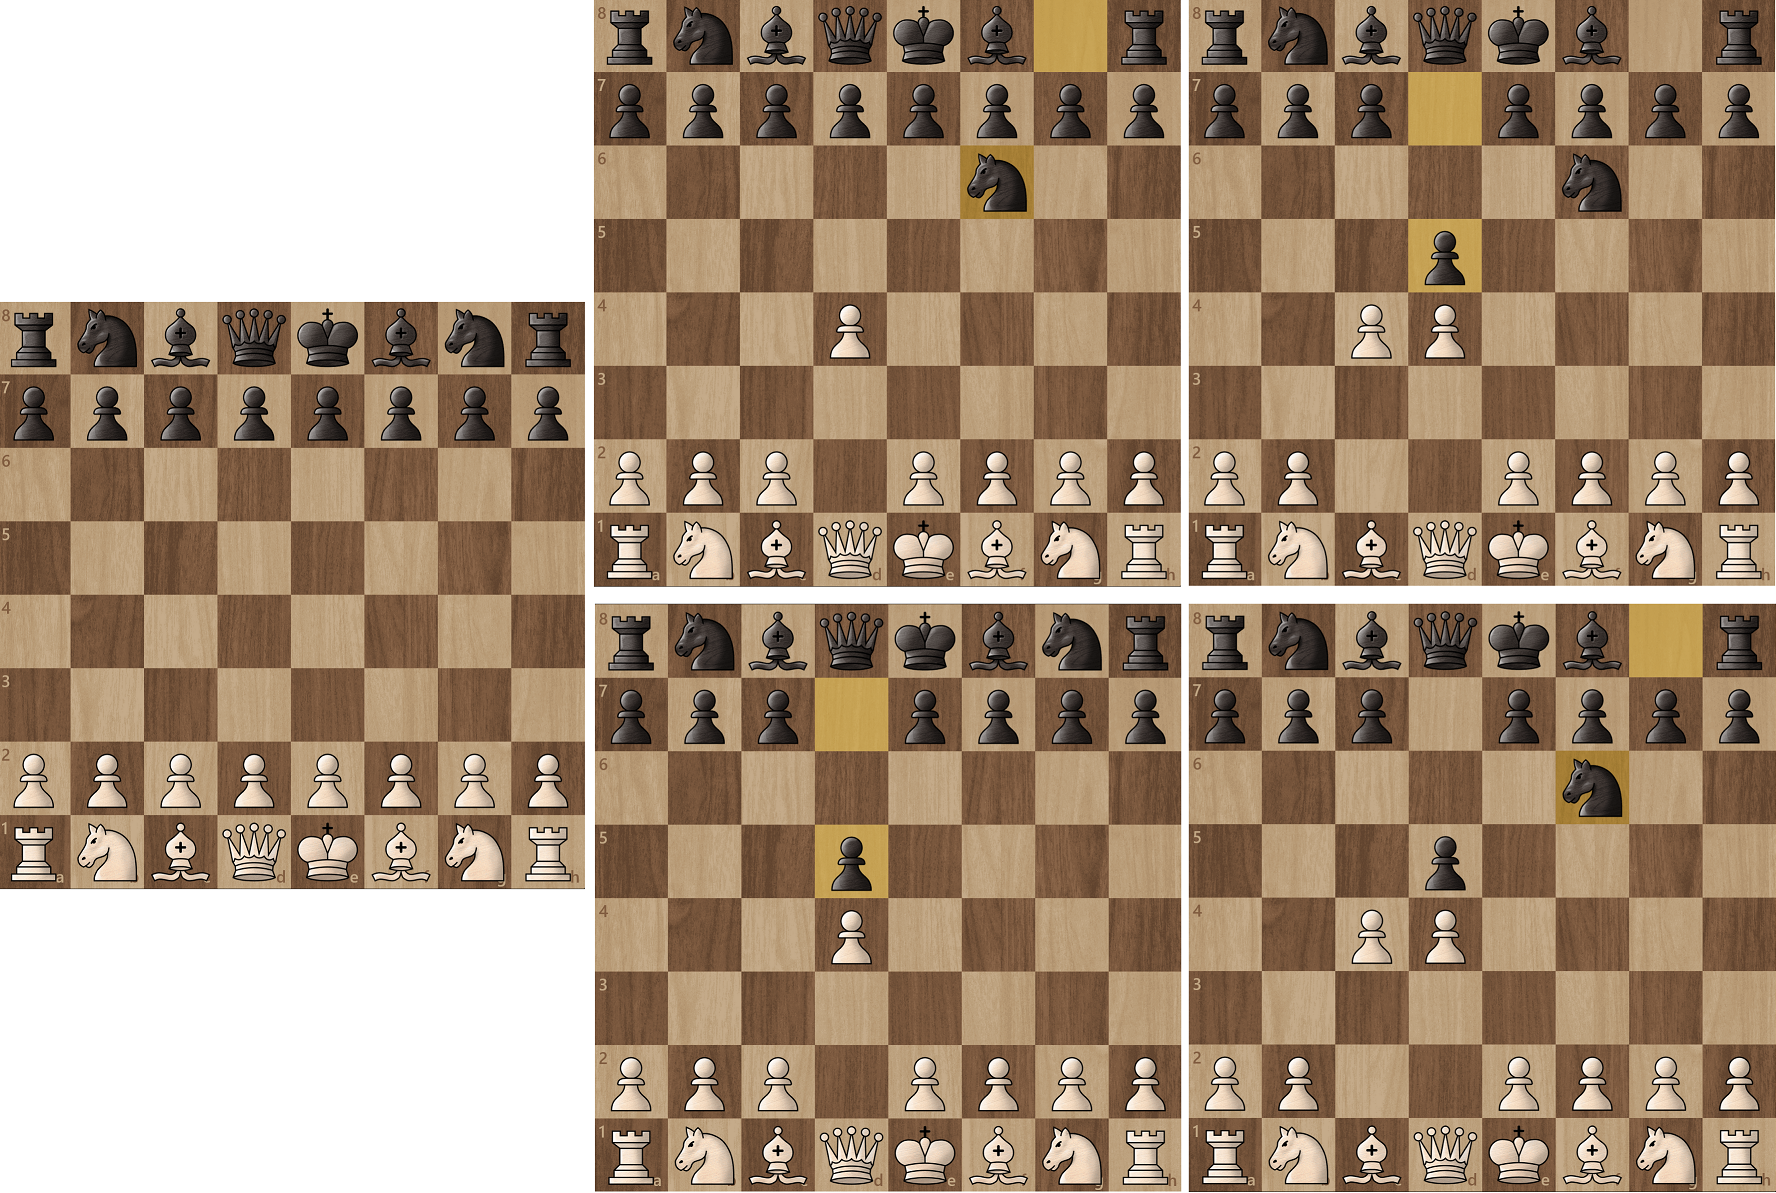
\includegraphics[scale=0.3]{images/transposition_example.png}
    \caption{Beispiel einer Transposition}
\end{figure}

Das Beispiel zeigt eine Stellung in einer Schacheröffnung. Trotz unterschiedlicher Reihenfolge der Züge des schwarzen Spielers, kommt es zur gleichen Endposition.
In komplexeren Stellungen kann diese Erkenntnis zu großen Zeitersparnissen führen.

Die Hauptidee hinter einer Transpositionstabelle ist, die Bewertung einer Position zu speichern, sobald sie berechnet wird. 
Die Bewertung zusammen mit der Position selbst wird in einer Tabelle gespeichert. 
Wenn später die gleiche oder eine transponierte Position auftritt, kann die Engine die Bewertung in der Transpositionstabelle nachschlagen, 
anstatt sie erneut zu berechnen.~\cite{Jos_W._H_1970_researchgate}

\subsubsection{Speicherung und Abfrage von zuvor berechneten Positionen}
Transpositionstabellen werden in Verbindung mit dem Suchalgorithmus des Computers verwendet. 
Wenn die Engine sich für den besten Zug entscheidet, durchsucht sie den Spielbaum, welcher eine Darstellung aller möglichen 
Zugsequenzen von der aktuellen Position aus ist. 
Wenn die Engine eine Position bewertet, überprüft sie zuerst, ob die Bewertung der Position in der Transpositionstabelle gespeichert ist. 
Falls ja, wird die gespeicherte Bewertung verwendet. Falls nicht, berechnet der Motor die Bewertung, 
speichert sie in der Tabelle und setzt dann die Suche fort.~\cite{Jos_W._H_1970_researchgate}

\subsection{Spielphasen}
Das Schachspiel wird in drei verschiedene Phasen unterteilt. Jede Phase hat dabei unterschiedliche Merkmale und Strategien, jedoch sind die Übergänge fließend.

\subsubsection{Eröffnung}
Die Eröffnungsphase des Spiels bezieht sich auf die anfänglichen Züge. Diese Phase ist entscheidend, um die Positionen der Spieler auf dem Brett zu etablieren, 
die Kontrolle über zentrale Felder zu gewinnen, den König in Sicherheit zu bringen und die Entwicklung der Figuren zu fördern. 
Es gibt zahlreiche gut dokumentierte Eröffnungsstrategien und Engines haben eine umfangreiche Bibliothek von Eröffnungszügen. 
Die Engine kann diese vorberechneten Züge verwenden, um sich durch die Eröffnungsphase zu navigieren, wodurch die Rechenzeit reduziert 
und ein starker Start gewährleistet wird.

\subsubsection{Mittelspiel}
Das Mittelspiel beginnt in der Regel, wenn die Spieler ihre anfängliche Figurenentwicklung abgeschlossen haben. 
Es ist gekennzeichnet durch dynamisches Spiel, bei dem strategische Planung, taktische Berechnungen und positionsbezogene Überlegungen eine wesentliche Rolle spielen. 
In dieser Phase führen die Computer eine umfassende Suche und Bewertung der möglichen Züge durch. 
Dieser Suchprozess beinhaltet oft Techniken wie Alpha-Beta-Pruning und die Verwendung von Transpositionstabellen, wie zuvor diskutiert. 
Die Entscheidungen, die in dieser Phase getroffen werden, beeinflussen die Spielrichtung erheblich und bereiten entweder einen entscheidenden Angriff 
oder ein ausgeglichenes Endspiel vor.

\subsubsection{Endspiel}
Die Endspielphase eines Schachspiels beginnt, wenn die meisten Figuren geschlagen wurden und überwiegend Könige und Bauern, zusammen mit wenigen anderen Figuren, 
auf dem Brett sind. Diese Phase ist in der Regel weniger taktisch als das Mittelspiel, beinhaltet aber komplexe strategische Überlegungen 
in Bezug auf Bauernstrukturen, Königsaktivitäten und Koordination der Figuren. 
Präzises Spiel ist in dieser Phase entscheidend, da ein Fehler das Ergebnis drastisch verändern kann. 
Engines nutzen Endspiel-Datenbanken, die perfekte Spielinformationen für alle Positionen mit einer geringen Anzahl von Figuren enthalten, 
um ein optimales Spiel in dieser Phase zu gewährleisten.

Jeder Spielphase hat unterschiedliche Herausforderungen, die von dem Computer gemeistert werden müssen. Die Eröffnung erfordert Kenntnisse der 
Eröffnungsprinzipien und eine umfangreiche Eröffnungsbibliothek, das Mittelspiel wird durch effiziente Suchalgorithmen und effektive Bewertungsfunktionen
entschieden und das Endspiel wird durch Endspiel-Datenbanken und spezielle Taktiken gewonnen.

\section{Schachcomputer auf Basis von maschinellem Lernen}

\subsection{Definition}
Schachcomputer, die auf maschinellem Lernen basieren, repräsentieren einen bedeutenden Fortschritt im Bereich der Schachinformatik. 
Diese Bots verwenden eine Reihe von Techniken des maschinellen Lernens, hauptsächlich das sogenannte Reinforcement Learning, 
um das Schachspiel zu verstehen und zu meistern. Im Gegensatz zu den traditionellen Engines stützen sich Schachcomputer, die auf maschinellem Lernen basieren, 
nicht ausschließlich auf handgemachte Evaluierungsfunktionen oder Algorithmen zur Zug-Generierung. 
Stattdessen lernen sie durch die Erfahrung des Spiels und optimieren ihre Strategien im Laufe der Zeit.~\cite{doi:10.1126/science.aar6404}

Ein prominentes Beispiel für einen Schachcomputer, der auf maschinellem Lernen basiert, ist DeepMinds AlphaZero, 
welches beispiellose Fähigkeiten im Bereich der Schach-KI zeigte. AlphaZero verwendet eine Variante der Monte Carlo Tree Search 
in Kombination mit tiefen neuronalen Netzwerken. Die neuronalen Netzwerke, die durch Selbstspiel und ohne Zugang zu existierendem Schachwissen trainiert wurden, 
leiten den Suchprozess, um vielversprechendere Züge zu erkunden. Mit der Zeit hat AlphaZero nicht nur alle traditionellen Schach-Engines übertroffen, 
sondern auch Strategien und Taktiken entdeckt, die neue Einblicke in das Spiel bieten.~\cite{David_Silver_2023_deepmind}

\subsection{Monte Carlo Tree Search}
Die Monte Carlo Tree Search ist eine suchbasierte KI-Methode, die in Spielen wird, bei denen der mögliche Zustandsraum enorm groß ist 
und daher eine vollständige Suche praktisch unmöglich ist. Die Monte Carlo Tree Search hat vier Hauptphasen: Auswahl, 
Expansion, Simulation und Rückwärtspropagation.~\cite{Ziad_Salloum_2019_towardsdatascience}

\subsubsection{Auswahl}
Startend an der aktuellen Spielposition navigiert der Algorithmus den Spielbaum unter Verwendung einer bestimmten Strategie, 
um den besten unterbewerteten Knoten zu finden.~\cite{Ziad_Salloum_2019_towardsdatascience}

\subsubsection{Expansion}
Sobald ein Knoten ausgewählt wurde, werden ein oder mehrere Kindknoten hinzugefügt, um mögliche Züge darzustellen.~\cite{Ziad_Salloum_2019_towardsdatascience}

\subsubsection{Simulation}
Vom expandierten Knoten aus wird eine zufällige Simulation des Spiels ausgeführt. Dies könnte so einfach sein wie das zufällige 
Spielen von Zügen bis zum Ende des Spiels.~\cite{Ziad_Salloum_2019_towardsdatascience}

\subsubsection{Rückwärtspropagation}
Nach der Simulation wird das Ergebnis auf alle Knoten in dem Pfad vom ausgewählten Knoten zurück zur Wurzel gegeben.

Dieser Prozess wird dann iterativ fortgesetzt, wobei jeder Durchlauf eine Suche darstellt, bis eine vordefinierte Bedingung erreicht ist, 
wie z.B. eine bestimmte Anzahl von Durchläufen, eine bestimmte Zeitgrenze oder eine ausreichende Gewissheit über den besten Zug.

Eine der Stärken vom \ac{MCTS} ist, dass er nicht auf heuristische Bewertungen der Spielpositionen angewiesen ist, 
wie es bei traditionellen suchbasierten Algorithmen der Fall ist. Stattdessen basiert \ac{MCTS} auf statistischen Analysen von simulierten Spielen, 
was dazu führt, dass sie oft unkonventionelle oder kreative Spielstrategien findet. Außerdem kann \ac{MCTS} auch in Spielen mit hohen 
Verzweigungsfaktoren effektiv eingesetzt werden, da sie durch die Verwendung von Simulationen die Notwendigkeit, 
den gesamten Spielbaum zu analysieren, umgeht.~\cite{Ziad_Salloum_2019_towardsdatascience}

\subsection{Übergang von nicht-maschinellem Lernen zu Schachcomputern auf Basis von maschinellem Lernen}
Der Übergang von Schachcomputern, die nicht auf maschinellem Lernen basieren, zu solchen, die es tun, 
markiert eine entscheidende Veränderung in der Herangehensweise an die Schachinformatik. 
Traditionell wurden Schachcomputer um die Prinzipien der Brute-Force-Suche und Bewertung, 
handgemachte Heuristiken und eine umfangreiche Bibliothek von Eröffnungs- und Endspielzügen herum entworfen. 
Während diese Engines eine hohe Leistung erzielten, waren sie aber durch die Tiefe ihrer Suche und die Qualität ihrer Heuristiken begrenzt.

Andererseits verwenden Bots, die auf maschinellem Lernen basieren, Algorithmen, um aus ihren Erfahrungen zu lernen, 
ihre Strategien anzupassen und ihr Spiel autonom zu verbessern. Dieser Lernprozess ermöglicht es ihnen, 
die Einschränkungen von handgemachten Heuristiken zu überwinden und flexiblere und effiziente Strategien zu erstellen.

Diese Veränderung wurde durch Fortschritte in der Rechenleistung, der Verfügbarkeit von Daten und den Algorithmen des maschinellen Lernens ermöglicht. 
Sie führt jedoch auch neue Herausforderungen und Überlegungen ein, wie die Interpretierbarkeit der von maschinellem Lernen getroffenen Entscheidungen 
und die für das Training solcher Modelle benötigten Rechenressourcen.~\cite{Demis_Hassabis_2017_nature}
    %!TEX root = ../dokumentation.tex

\chapter{Diskussion über die Benutzeroberfläche und Programmiersprache}
Dieses Kapitel beschäftigt sich  mit den relevanten Entscheidungen, die hinter dem Aufbau und der Implementierung der Anwendung stehen. 
Die zentralen Auswahlkriterien, wie die verwendete Programmiersprache und die verwendeten Softwarebibliotheken, 
bestimmen in hohem Maße die Eigenschaften und Fähigkeiten des Programms.

Zunächst wird die Begründung für die Auswahl von Python als bevorzugter Sprache analysiert, 
wobei Alternativen wie Java und C++ in Betracht gezogen werden. Danach rückt die Untersuchung der während der Entwicklungsphase 
des Projekts genutzten Bibliotheken in den Fokus. Pygame wird für die Erstellung der Spielumgebung verwendet und OpenCV für die Bildverarbeitung. 
Die Vor- und Nachteile jeder Bibliothek werden gegen potenzielle Alternativen abgewogen und geben umfassende Einblicke in den Entscheidungsprozess.

Außerdem beschäftigt sich das Kapitel mit dem \ac{UI} Designs und der \ac{UX}, 
Prinzipien, die die Benutzerbindung und -zufriedenheit steigern. Diese Komponenten sind für den Erfolg jeder Anwendung unerlässlich, 
insbesondere in interaktiven Umgebungen wie einem Spiel.

Der abschließende Abschnitt fasst die Diskussionen zusammen und bekräftigt die Begründungen für die Auswahl, indem er reflektiert, 
wie diese Entscheidungen es ermöglicht haben, die funktionalen Anforderungen der Anwendung zu erfüllen und gleichzeitig ein 
zufriedenstellendes Benutzererlebnis zu gewährleisten.

\section{Auswahl der Programmiersprache}
Eine der grundlegendsten Entscheidungen bei der Entwicklung von Software ist die Wahl der Programmiersprache. 
Die Entscheidung für Python wurde durch eine Reihe von Faktoren beeinflusst, welche im Folgenden aufgezeigt werden. 
Jede Programmiersprache hat Stärken und Schwächen und die Wahl hängt von den spezifischen Anforderungen des Projekts ab.

\subsection{Python}
Python, die für dieses Projekt gewählte Sprache, ist eine High-Level-Interpretersprache, die für ihre Einfachheit und Benutzerfreundlichkeit bekannt ist.
Sie wird zunehmend für eine breite Palette von Anwendungen eingesetzt, von der Web- und Spieleentwicklung,
bis hin zum maschinellen Lernen und der wissenschaftlichen Datenverarbeitung.

\subsubsection{Vorteile von Python}
\paragraph{Einfache Syntax}
Die Syntax von Python ist so gestaltet, dass sie lesbar und unkompliziert ist. 
Die Sprache bietet klaren, logischen, Code für Projekte jeder Größe.

\paragraph{Umfangreiche Bibliotheksunterstützung}
Python ist bekannt für seine umfangreiche Bibliotheksunterstützung, die komplexe Aufgaben vereinfacht. 
Bibliotheken wie Pygame für die Spieleentwicklung und OpenCV für die Computer Vision haben die Entwicklungszeit für dieses Projekt erheblich reduziert.

\paragraph{Gemeinschaft und Ressourcen}
Mit einer großen und aktiven Community bietet Python viele von Ressourcen und Hilfestellungen. 
Die Open-Source-Natur von Python verbessert die Verfügbarkeit von Codebasen für die Programmierung. 
Dies, gepaart mit einer großen Anzahl von Tutorials und Dokumentationen, macht Python zu einer attraktiven Option für Entwickler.

\paragraph{Python und Schachprogrammierung}
Python hat ebenfalls einen Einsatz in der Schachprogrammierung gefunden. 
Engines wie Stockfish haben Implementierungen in Python. Die Flexibilität von Python und die einfache Erstellung von Prototypen 
machen es geeignet für die iterative Natur der Spieleentwicklung.

\subsubsection{Nachteile von Python}
\paragraph{Geschwindigkeit}
Die Ausführungsgeschwindigkeit von Python ist langsamer als bei kompilierten Sprachen wie C++ oder Java. 
Dies liegt daran, dass Python eine interpretierte Sprache ist, was bedeutet, dass sie Code Zeile für Zeile ausführt, 
was langsamer ist als andere Sprachen, die das gesamte Programm vor der Ausführung kompilieren.

\paragraph{Speicherverbrauch}
Auch der Speicherverbrauch von Python ist höher als bei anderen Sprachen.
Python verwendet dynamische Typisierung. Das heißt, dass Variablentypen nicht explizit vom Programmierer deklariert werden. 
Stattdessen wird der Typ zur Laufzeit bestimmt. In einer dynamisch typisierten Sprache kann jeder Variable jeder Typ zugewiesen werden. 
Zum Beispiel kann einer Variable, der anfangs ein String-Wert zugewiesen wird, später ein Integer oder ein Boolean zugewiesen werden.
Deshalb verwendet Python mehr Speicher, was zu Problemen führen kann.

\subsubsection{Verwendung in der Industrie}
Obwohl Python für Entwicklung und Prototyping beliebt ist, wird es in der Spieleindustrie nicht so weit verbreitet eingesetzt wie C++. 
Dies ist zum Teil auf die langsamere Geschwindigkeit und den höheren Speicherverbrauch zurückzuführen.

Zusammenfassend lässt sich sagen, dass Python für dieses Projekt aufgrund seiner Lesbarkeit, 
umfangreichen Bibliotheksunterstützung und der aktiven Community gewählt wurde. 
Trotz seiner Nachteile überwogen die Vorteile für die spezifischen Anforderungen dieser Anwendung.

\subsection{Alternativen zu Python}
Im Bereich der Programmierung gibt es eine Vielzahl von Sprachen, die genutzt werden können und jeweils 
einzigartige Stärken und Schwächen aufweisen. Obwohl sich für Python entschieden wurde, standen auch Java und C++
zur Debatte.

\subsubsection{Java}
Java ist seit langem ein fester Bestandteil in der Softwarebranche aufgrund ihrer plattformunabhängigen Natur, die durch die \ac{JVM} ermöglicht wird. 
Das bedeutet, dass ein Java-Programm auf jedem Gerät laufen kann, das eine \ac{JVM} hat, was zum Erfolg von Java über Plattformen hinweg beiträgt.

Die Vorteile von Java sind Robustheit, Plattformunabhängigkeit und eine umfangreiche Standardbibliothek, ähnlich wie bei Python. 
Es ist statisch typisiert, was mehr Sicherheit zur Kompilierzeit bietet. Darüber hinaus ist Java schneller als Python, da der Java-Code in 
Bytecode kompiliert wird und auf der \ac{JVM} läuft, ein Merkmal, das Java einen Vorteil bei Anwendungen bietet, die eine hohe Leistung erfordern.

Im Kontext der Schachprogrammierung kann die hohe Ausführungsgeschwindigkeit von Java zu effizienteren Suchalgorithmen und KI-Logik führen. 
Die Java-Syntax kann jedoch den Programmierprozess mühsamer machen und die Entwicklung von GUIs kann im Vergleich zu Python komplexer sein.

\subsubsection{C++}
C++ ist bekannt für ihre hohe Leistung und die Kontrolle über Systemressourcen. 
Sie wird häufig in Anwendungen eingesetzt, bei denen die Leistung kritisch ist, wie zum Beispiel in der Spieleentwicklung, 
in Betriebssystemen und in Echtzeitsystemen.

In der Schachprogrammierung kann C++ eine überlegene Leistung bieten und ermöglicht tiefere Suchen im Spielbaum innerhalb der gleichen Zeitspanne. 
Es ermöglicht auch Manipulationen auf niedrigerer Ebene, was beim Optimieren von Speicher und Rechenressourcen von Vorteil sein kann.
Die Speicherverwaltung in C++ ist manuell und kann zu Fehlern führen, die schwer zu entdecken sind.

\subsection{Vergleich von Python, Java und C++}
Obwohl alle drei Sprachen erfolgreich in der Schachprogrammierung eingesetzt wurden, können ihre Unterschiede in Syntax, 
Leistung und Nutzungsphilosophie zu unterschiedlichen Erfahrungen im Entwicklungsprozess führen. 
Python, mit seinem Fokus auf Code-Lesbarkeit und Einfachheit, führt zu schnelleren Entwicklungszyklen, 
kann jedoch in Bezug auf die Leistung hinterherhinken. Java und C++ bieten bei höherer Komplexität eine bessere Leistung.

Die Wahl der richtigen Sprache für ein Projekt hängt von den spezifischen Bedürfnissen und Einschränkungen des Projekts, 
der Vertrautheit des Entwicklungsteams mit der Sprache und den Anforderungen an Leistung und Plattformkompatibilität ab.

\section{Diskussion über Bibliotheken/Frameworks}
\subsubsection{Pygame}
Pygame ist eine Open-Source Python-Bibliothek, die für die Erstellung von Videospielen konzipiert ist. 
Sie basiert auf der \ac{SDL} und läuft auf fast jeder Plattform und jedem Betriebssystem.

Einer der Hauptvorteile von Pygame ist seine Einfachheit.
Pygame ist sehr flexibel, was dem Entwickler eine vollständige Kontrolle über den Spielentwicklungsprozess ermöglicht. 
Darüber hinaus verfügt es über eine große und aktive Community, die eine Vielzahl von Ressourcen, Tutorials und Anleitungen bereitstellt, 
die den Entwicklungsprozess weiter unterstützen.

\subsubsection{OpenCV}
OpenCV ist eine Open-Source Bibliothek für Computer Vision und maschinelles Lernen. 
Sie enthält eine Vielzahl an Algorithmen für Bildanalyse, Videoanalyse und Objekterkennung.

Der Funktionsumfang macht es für fast jede Aufgabe der Computer Vision geeignet. 
Es ist auf Recheneffizienz ausgelegt, mit einem starken Fokus auf Echtzeitanwendungen. 
Da es sich um ein Open-Source-Projekt handelt, gibt es eine große Community von Entwicklern, 
die kontinuierlich an Verbesserungen und Updates arbeiten und so eine starke Unterstützung bieten.

Auf der anderen Seite steigt mit der Funktionalität auch die Komplexität. Obwohl es eine Vielzahl von Funktionen bietet, 
kann die Nutzung dieser Funktionen kompliziert sein und das tiefgreifende Verständnis der Bibliothek erfordert einen erheblichen Aufwand und Zeit.

\subsubsection{Alternativen zu Pygame und OpenCV}
Neben Pygame und OpenCV, gibt es zahlreiche andere Bibliotheken und Frameworks, die für die Spielentwicklung und 
Bildverarbeitungsaufgaben verwendet werden könnten. Beispielsweise sind Unity und Unreal Engine leistungsstarke Engines, 
aber sie sind komplexer und erfordern eine erhebliche Lerninvestition. 
Im Bereich der Bildverarbeitung und Computer Vision könnten auch Bibliotheken wie die Python Imaging Library oder SciKit-Image verwendet werden, 
obwohl sie möglicherweise nicht die gleiche Breite an Funktionen wie OpenCV bieten.
Die Wahl der Bibliothek oder des Frameworks hängt von verschiedenen Faktoren ab, einschließlich der spezifischen Anforderungen des Projekts, 
der Vertrautheit der Entwickler mit den Tools und dem gewünschten Gleichgewicht zwischen Benutzerfreundlichkeit und Funktionalität.

Aufgrund der einfachen Implementierung wurde sich in diesem Projekt für Pygame entschieden. OpenCV wurde aufgrund von Vorwissen und Vertrautheit gewählt.

\section{Benutzeroberfläche und Benutzererfahrung}
Das \ac{UI} und die \ac{UX} sind entscheidende Aspekte jeder Anwendung. Eine ansprechende, intuitive und benutzerfreundliche Umgebung 
kann den Unterschied ausmachen zwischen einer Anwendung, die schnell verworfen wird, und einer, die regelmäßig genutzt und weiterempfohlen wird.

\subsubsection{Bedeutung einer benutzerfreundlichen Umgebung}
Bei der Erstellung einer Schachanwendung ist die Zugänglichkeit ein wesentlicher Aspekt. Eine benutzerfreundliche Oberfläche, 
die leicht navigierbar ist und deutlich beschriftete Optionen und Werkzeuge aufweist, ermöglicht es Spielern, 
effizient und effektiv mit dem Spiel zu interagieren. Darüber hinaus spielt die Zugänglichkeit eine wichtige Rolle bei der Gewährleistung, 
dass die Anwendung für alle potenziellen Nutzer zugänglich ist.

Die Nutzerzufriedenheit ist ein entscheidender Faktor, der untrennbar mit einer benutzerfreundlichen Umgebung verbunden ist. 
Wenn Nutzer die Anwendung als schwer zu bedienen oder zu navigieren empfinden oder wenn sie ihren Erwartungen hinsichtlich 
Funktionalität und Ästhetik nicht entspricht, führt das unweigerlich zu Unzufriedenheit. 
Diese Unzufriedenheit kann zu negativen Bewertungen und Feedback führen, was die Reputation und 
Nutzerbasis der Anwendung beeinträchtigen kann.

\subsubsection{Designprinzipien für eine benutzerfreundliche Umgebung}
\paragraph{Einfachheit}
Eine Benutzeroberfläche sollte so einfach wie möglich sein und den Benutzern nur die notwendigen Funktionen zur Verfügung stellen, 
um ihre Aufgaben zu erfüllen. Dies bedeutet nicht, die Anwendung von nützlichen Funktionen zu befreien, sondern diese so zu präsentieren, 
dass sie den Benutzer nicht überfordern.

\paragraph{Konsistenz}
Konsistenz in Designelementen wie Schriftarten, Farben und Layout reduziert die Lernkurve für Benutzer. 
Es ermöglicht ihnen, sich schnell mit der Benutzeroberfläche vertraut zu machen, was zu einer und intuitiven Benutzererfahrung führt.
 
\paragraph{Rückmeldung und Reaktionszeit}
Benutzern sollte eindeutiges Feedback zu ihren Aktionen gegeben werden. 
Wenn beispielsweise ein Benutzer einen Zug in einem Schachspiel macht, sollte die Anwendung schnell reagieren und die Ergebnisse dieses Zuges anzeigen. 
Verzögertes oder unzureichendes Feedback kann zu Benutzerfrustration und Verwirrung führen.~\cite{Uxpin_2022_uxpin}

\paragraph{Benutzerkontrolle}
Benutzer sollten das Gefühl haben, die Anwendung zu kontrollieren. Dies kann erreicht werden, indem Benutzern erlaubt wird, 
Aktionen einfach rückgängig zu machen und zu wiederholen, sich frei innerhalb der Anwendung zu bewegen und 
Einstellungen nach ihren Vorlieben anzupassen.~\cite{Uxpin_2022_uxpin}

\section{Schlussfolgerung}
Aufgrund der einfachen Erstellung von Prototypen, die eine iterative Arbeitsweise fördern, 
wurde sich in diesem Projekt für Python als Programmiersprache entschlossen. Die schwächere Leistung ist zwar bemerkbar, jedoch immernoch 
gut genug um die Ziele dieses Projektes zu erreichen.

Aufgrund der Implementierung von Python wurde sich für die Nutzung von Pygame als Game-Engine entschieden, um schnell und unkompliziert 
Prototypen zu erstellen, die der Grund für die Wahl der Programmiersprache waren.

Die Verbindung zur Kamerafunktionalität ist im Projekt mittels OpenCV verankert, da hier, im Gegensatz zu anderen Moeglichkeiten, schon Vorkenntnisse 
herrschen.


	%!TEX root = ../dokumentation.tex

\chapter{Erstellung der Anwendung}
In den vorherigen Kapiteln wurden grundlegende Ansätze der digitalen Bildverarbeitung und Schach-Engines erläutert.
Dieses Kapitel beschäftigt sich mit der Implementierung des gewonnenen Wissens, um das Ziel der Applikation zu erreichen.  
Es wird aufgezeigt, wie das Projekt über einen objektorientierten Ansatz und mithilfe von Pygame zur 
Erstellung des Spiels, sowie OpenCV zur Kameraauswertung, umgesetzt wurde.

\section{Design und Architektur}
Das Projekt verfolgt einen objektorientierten Ansatz. Es existieren sieben Hauptklassen und eine Klasse für Konstanten.
Im Folgenden werden die Klassen und deren Aufgabe in Bezug auf die Applikation aufgeführt.

\subsection{Figuren Klasse}
Die Figuren Klasse stellt eine Schachfigur dar. Dabei hat jede Figur eine \(COLOR\), die entweder schwarz oder weiß ist.
Die weiße Farbe wird dabei mit \(0b0\) dargestellt und die schwarze Farbe mit \(0b1\). Dieses Farbschema zieht sich über das komplette Projekt.
Neben der Farbe hat jede Figur einen Namen, der dem Namen der jeweiligen Bilddatei entspricht. Ein weißer Bauer hat also den Namen \(0\_pawn.png \).  
Der Parameter \(TYPE\) ist ein String, der den Figurentyp beschreibt.

\begin{itemize}
    \item {\(p\) beschreibt einen Bauern.}
    \item {\(r\) beschreibt einen Turm.}
    \item {\(n\) beschreibt einen Springer.}
    \item {\(b\) beschreibt einen Läufer.}
    \item {\(q\) beschreibt eine Dame.}
    \item {\(k\) beschreibt einen König.}
\end{itemize}

Außerdem besitzt jede Figur eine Liste \(moves\), die alle legalen Züge der Figur beinhaltet. Die Züge sind Objekte einer Hilfsklasse, auf die später 
genauer eingegangen wird. Der Boolean \(HAS\_RANGE\_MOVEMENT\) gibt an, ob die Figur ein Läufer, Turm oder eine Dame ist. Wenn das der Fall ist,
ist der Wert wahr, ansonsten ist er falsch. Das letzte Attribut \(has\_moved\) beschreibt, ob eine Figur bereits gezogen wurde.
\begin{figure}[ht]
    \centering
    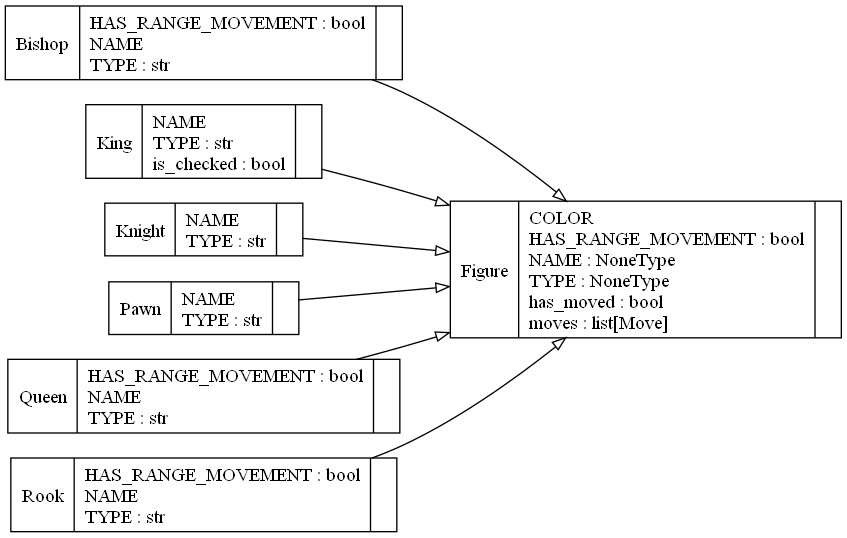
\includegraphics[scale=0.6]{images/classes_figures.png}
    \caption{Figuren Klassen}
\end{figure}
Neben der allgemeinen Figuren Klasse, gibt es für jede Figur noch eine einzelne Klasse, die jeweils von der Figuren Klasse erbt.
Um einen schwarzen Bauern zu erstellen, wird also ein Objekt mit dem Konstruktor der Bauern Klasse erstellt, die nur noch die Farbe als Parameter nimmt.
Die restlichen Attribute werden automatisch gesetzt. Der König hat dabei noch ein extra Attribut \(is\_checked\), das wahr wird, wenn er angegriffen wird.

\subsection{Schachbrett Klasse}
\begin{figure}[ht]
    \centering
    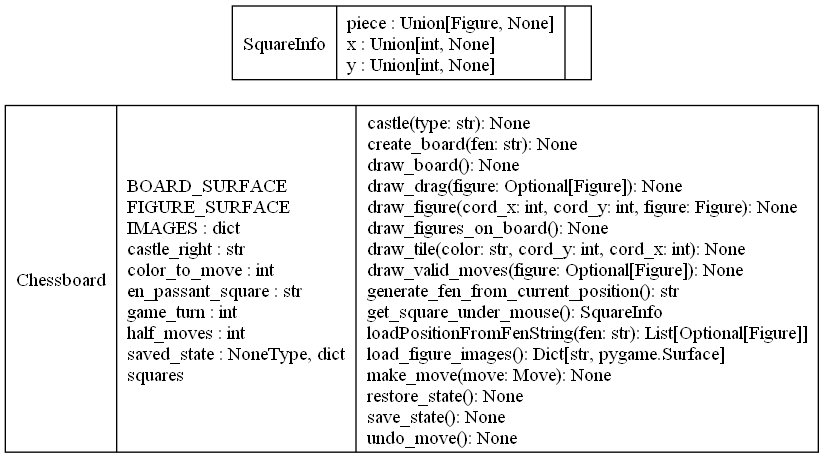
\includegraphics[scale=0.6]{images/classes_chessboard.png}
    \caption{Schachbrett Klasse}
\end{figure}
Die Klasse \(chessboard.py\) beinhaltet alle Attribute und Funktionen, die mit dem Schachbrett zu tun haben. Dazu gehört das Zeichnen des Schachbretts, 
das Zeichen der Figuren auf dem Schachbrett, das Speichern der aktuellen Position und das Spielen oder zurücknehmen von Zügen.

\subsection{Klasse zur Kameraimplementierung}
Die Klasse \(ChessCam.py\) dient dazu, mithilfe einer Kamera die Züge des Spielers zu erkennen. Es gibt eine Funktion, die das Schachbrett erkennt und 
Funktionen mit deren Hilfe die Unterschiede zu einer vorherigen Position ausgewertet werden, um dann den Spielzug zu erkennen.
\begin{figure}[ht]
    \centering
    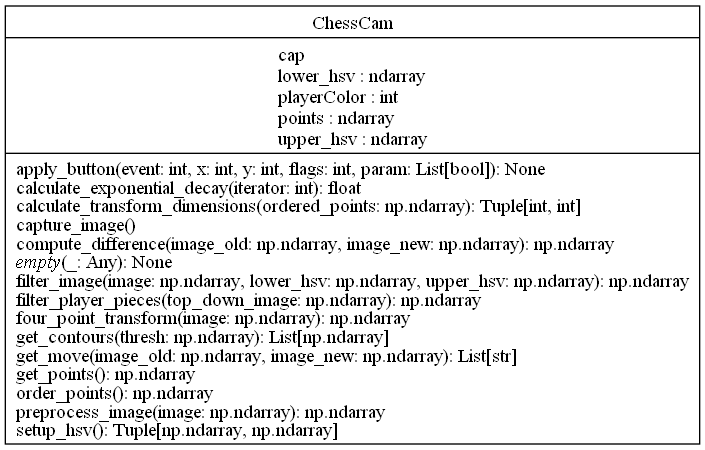
\includegraphics[scale=0.6]{images/class_cam.png}
    \caption{ChessCam Klasse}
\end{figure}

\subsection{Klasse zur Zuggenerierung}
\(moveGenerator.py\) dient dazu, die legalen Züge des aktuellen Spielers zu berechnen. Das ist notwendig, um dem Spieler die verfügbaren Züge anzuzeigen und 
illegale eventuell falsch erkannte Züge zu verbieten. Die legalen Züge werden anschließend der jeweiligen Figur als Attribut gegeben.
Sobald ein Spieler keinen legalen Zug mehr hat, ist das Spiel zu Ende und der andere Spieler gewinnt. Die generierten Züge sind dabei vom Datentyp \(Move\).

\subsection{Move Klasse}
\begin{figure}[H]
    \centering
    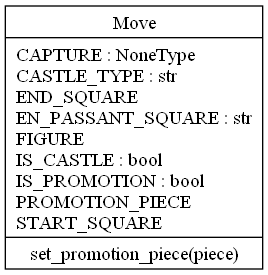
\includegraphics[scale=0.7]{images/class_move.png}
    \caption{Move Klasse}
\end{figure}

Diese Klasse dient als Hilfsklasse, um einen Zug zu beschreiben. Sie beinhaltet dabei das Startfeld, das Endfeld des Zuges, sowie die Figur, die den Zug ausführt.
Sollte es sich um einen Sonderzug handeln werden bestimmte flags gesetzt, die dies kennzeichnen. Ein Bauernzug, der zwei Felder nach vorne geht, beinhaltet
beispielsweise das \(EN\_PASSANT\_SQUARE\) flag.

\subsection{Computer Klasse}
Das Computer-Objekt wird genutzt, um die Züge der Engine zu berechnen. Dabei wird die Python Bibliothek von Stockfish genutzt, die die aktuelle Position 
als Input bekommt und dann anschließend einen Zug an die PyChess Klasse zurückgibt und dann auf dem Brett gespielt wird.

\subsection{PyChess Klasse}
Die Klasse \(pychess.py\) ist das Kernstück der Anwendung. In ihr wird das Spiel gestartet, das Schachbrett aus einer bestimmten Position gestartet,
und sie ist dafür verantwortlich, dass der Spieler mit der GUI interagieren kann, um seine Züge zu spielen.

\section{Spielverlauf}
\begin{figure}[H]
    \centering
    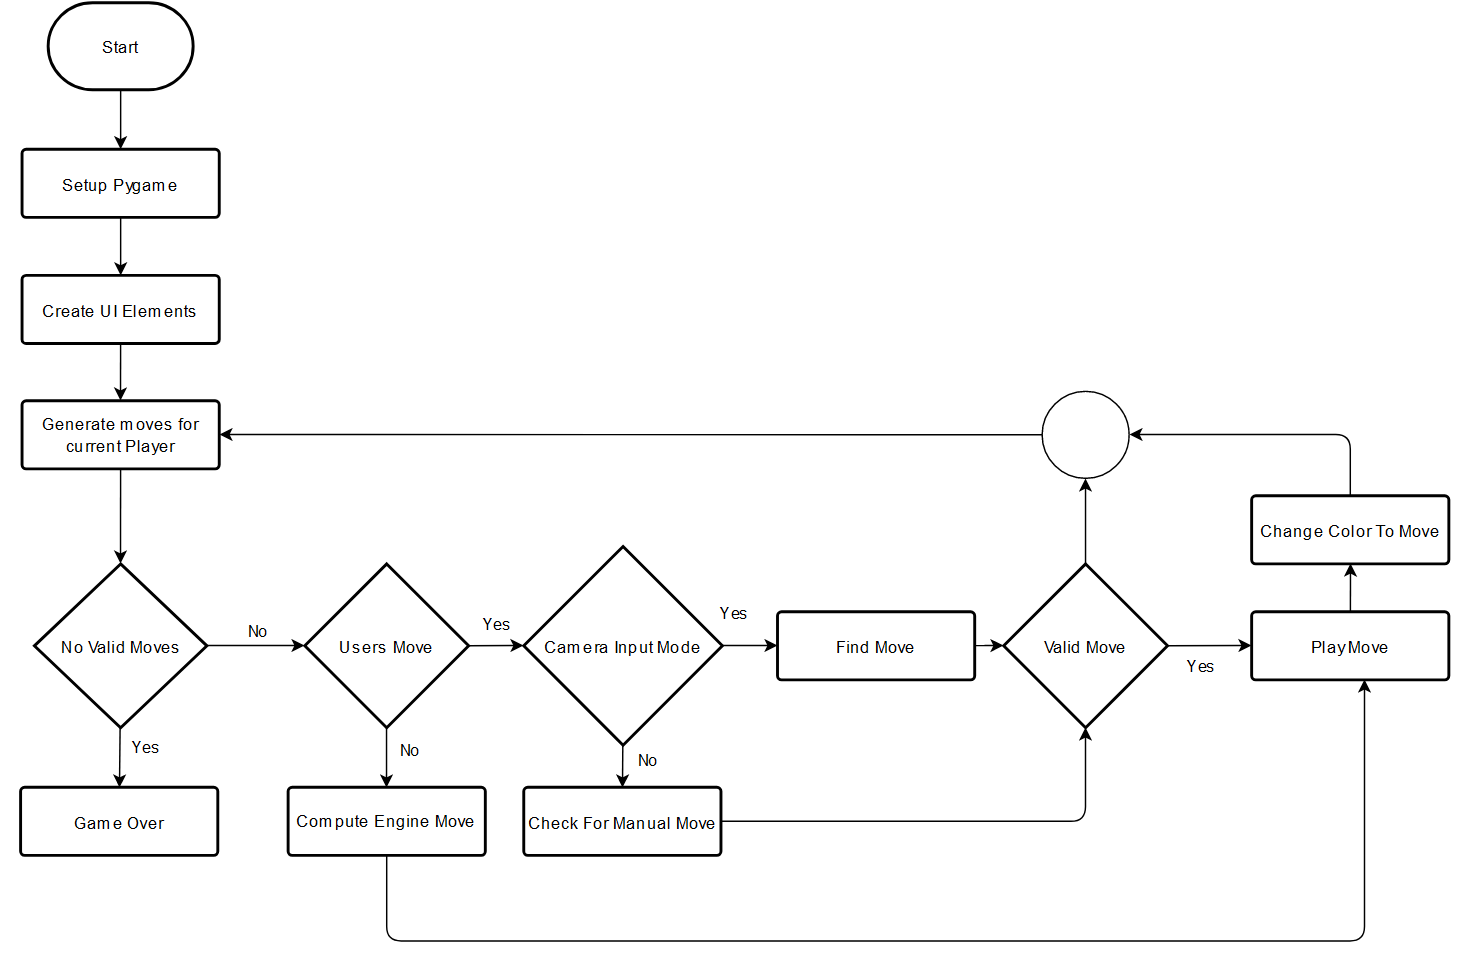
\includegraphics[scale=0.45]{images/game_loop_flowchart.png}
    \caption{PyChess Gameloop}
\end{figure}
\subsection{Voreinstellungen}
Nach Starten des Spiels wird das Spiel initialisiert. In dieser Initialisierung wird die Farbe des Spielers und des Computers bestimmt. 
Anschließend wird die Kamera des Nutzers aktiviert und der Nutzer kann die Ecken des Schachbretts markieren. Eine weitere Möglichkeit ist, das Schachbrett 
automatisch zu erkennen, jedoch wurde sich aufgrund von nachfolgenden Gründen dagegen entschieden.
\begin{figure}[H]
    \centering
    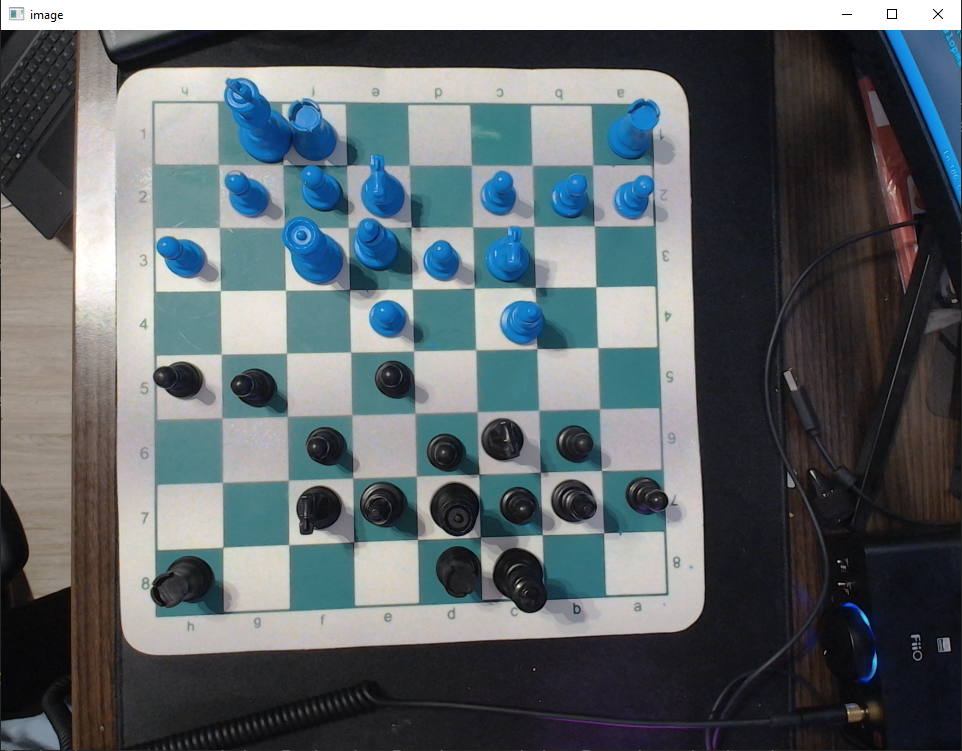
\includegraphics[scale=0.45]{images/scan_for_chessboard.png}
    \caption{Schachbrett markieren Dialog}
\end{figure}

Nachdem das Schachbrett markiert wurde, erscheint ein weiterer Dialog. In diesem wird einerseits das markierte Brett, sowie ein Dialog 
zum Einstellen der Farbregulierung angezeigt.
\begin{figure}[H]
    \centering
    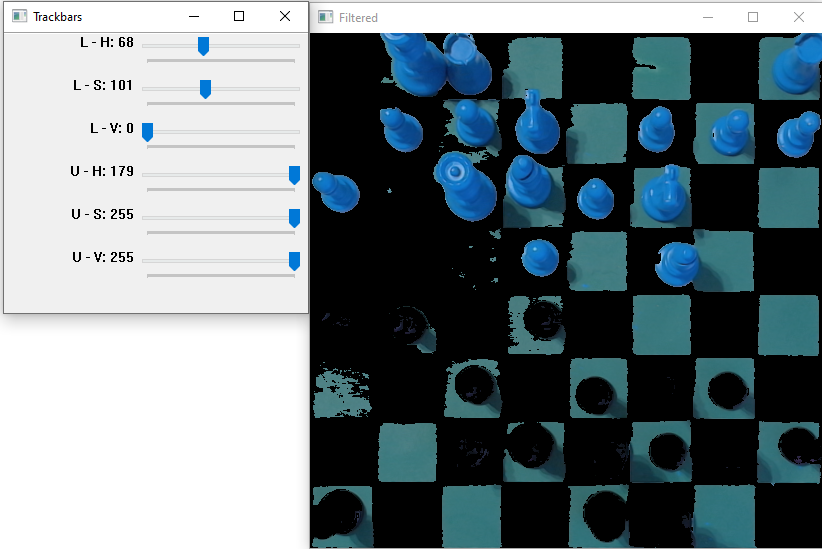
\includegraphics[scale=0.45]{images/color_filter_selection.png}
    \caption{Farbfilter Dialog}
\end{figure}

Mithilfe der Slidern, können die oberen und unteren Grenzen des HSV-Farbfilters gesetzt werden. Über das live Bild des Schachbretts wird angezeigt, wie sich die 
Einstellungen auswirken. Der Nutzer kann dann individuell auf das Schachbrett angepasst, die Werte so setzen, dass nur noch seine eigenen Spielfiguren zu sehen sind.
Dieser Schritt ist von großer Bedeutung für die spätere Zugerkennung.

Nachdem der Nutzer den Filter bestätigt hat, werden die restlichen \ac{UI} Elemente erstellt und die GUI angezeigt. 
\begin{figure}[H]
    \centering
    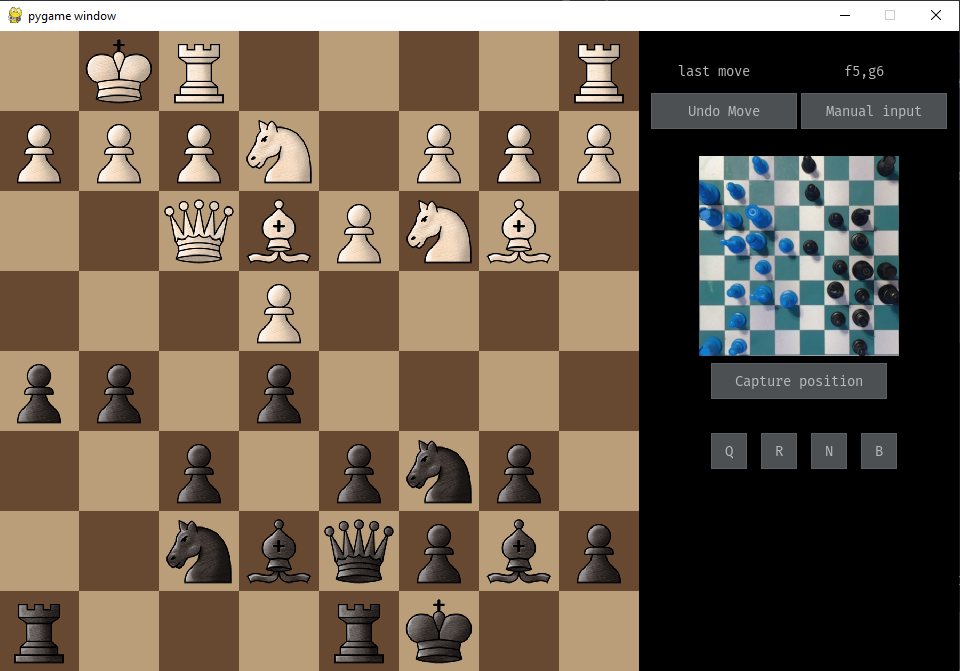
\includegraphics[scale=0.6]{images/pychess_window.png}
    \caption{PyChess Game GUI}
    \label{fig:PychessGUI}
\end{figure}

\subsection{Gameloop}
Ab hier beginnt die Gameloop. Am Anfang jeder Iteration werden alle validen Züge des aktuellen Spielers generiert und in einer Liste gespeichert.
Wenn diese Liste leer ist, also der Spieler keine Züge mehr hat, ist das Spiel zu Ende. 

\subsection{Zugerstellung}
Die Züge werden über die Funktion \(generate\_moves\) des \(moveGenerator\) Objekts erstellt.
\begin{figure}[H]
    \centering
    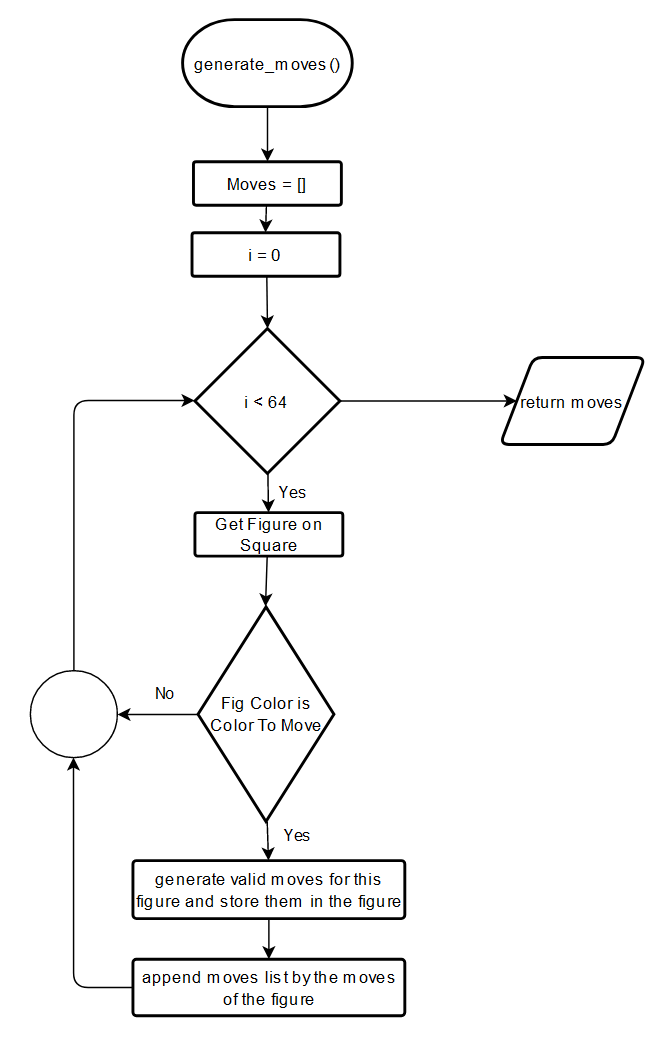
\includegraphics[scale=0.6]{images/generate_moves_function.png}
    \caption{Generierung der validen Spielzüge}
\end{figure}

Je nach Typ der Figur werden verschiedene Funktionen genutzt, um die validen Züge zu erstellen. Das Prozedere ist jedoch ähnlich.
Von einer Position ausgehend sind die Felder, auf die sich eine Figur bewegen kann immer einen bestimmten Offset entfernt.
Angenommen die aktuelle Figur ist ein König, der auf dem Feld 27 steht. Von diesem Feld ausgehend, haben die anliegenden Felder immer den gleichen Abstand in Bezug auf die Startposition.
\begin{figure}[H]
    \centering
    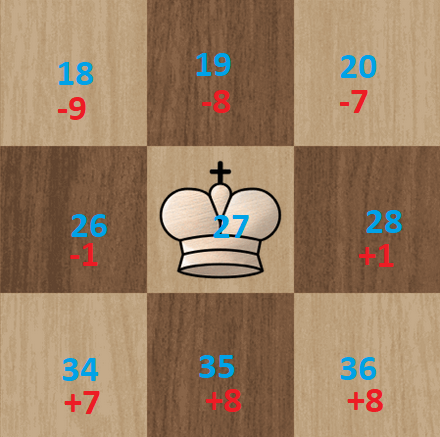
\includegraphics[scale=0.3]{images/offset_king.png}
    \caption{Figuren Offset König}
\end{figure}

Bei einem König sind damit alle vorerst validen Züge ausschließlich der Rochade abgedeckt. Bei Läufern, Türmen und Damen können die jeweiligen Offsets mit einer 
sich iterativ erhöhenden Anzahl an schritten multipliziert werden.
Springer haben einen anderen Offset als ein König, aber folgen demselben Prinzip. Nachdem diese Züge bestimmt wurden, wird ermittelt, ob der Zug legal ist.
Wenn eine eigene Figur das Feld belegt ist der Zug illegal und wird direkt verworfen und die Iteration für den Offset gegebenenfalls beendet. 
Wenn eine gegnerische Figur das Feld besetzt wird der Zug nicht direkt verworfen, aber die Iteration für das aktuelle Offset der jeweiligen Figuren beendet 
und der nächste Offset wird durchiteriert. 
Bei den Bauernzügen ist es wichtig, dass nur diagonal geschlagen werden kann und sich sonst nur ein Feld vorwärts bewegt werden kann.
Eine weitere Prüfung findet statt, ob der Zug am Ende des Brettes ist. Ohne diese Überprüfung wäre es möglich aus dem zum Beispiel linken Rand auszubrechen und rechts wieder
ins Spiel zu kommen.

\subsubsection{Spezialzüge}
Der erste Zug jedes Bauern ist hierbei eine Ausnahme, da er sich dort zwei Felder vorwärts bewegen kann. Das wird durch das Attribut \(has\_moved\) der Figur überprüft.
Der Spezialzug \(en~passant\) muss ebenfalls beachtet werden.
Dieser Tritt auf, wenn ein gegnerischer Bauer sich im letzten Zug zwei Felder nach vorne bewegt hat, und nun neben dem eigenen steht. Dann kann der gegnerische Bauer 
im Vorbeilaufen geschlagen werden. Das Feld, auf dem \(en~passant\) geschlagen werden kann wird nach jedem Zug in dem Schachbrett Objekt neu gesetzt.

\begin{figure}[H]
    \centering
    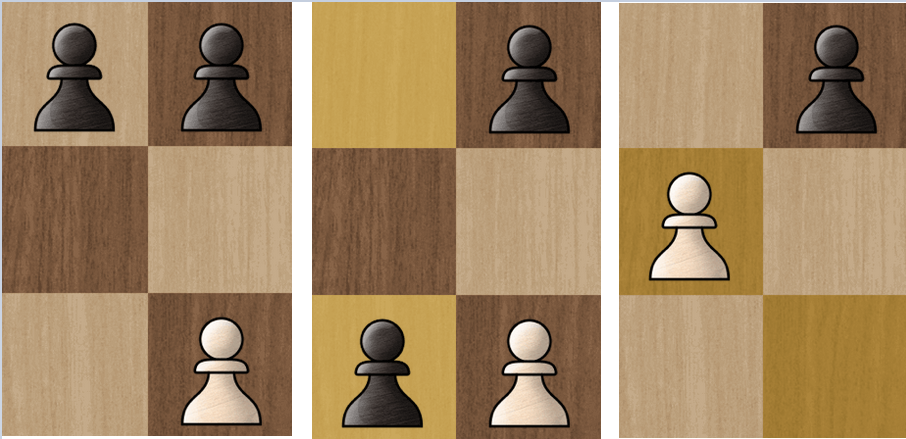
\includegraphics[scale=0.3]{images/en_passant.png}
    \caption{En Passant}
\end{figure}

Sollte ein Spieler mit dem Bauer auf die letzte Reihe kommen, kann er diesen zu einer beliebigen Figur, außer König und Bauer umwandeln.
Der letzte Spezialzug im Schach ist die Rochade, bei der ein Doppelzug von König und Turm vorliegt. Der König bewegt sich dabei zwei Felder in Richtung
des eigenen Turms und der Turm stellt sich hinter den König. Die Voraussetzungen hierfür sind, dass sich König und Turm nicht bewegt haben und der 
König nicht über ein Feld läuft, das vom Gegner kontrolliert wird. 

\begin{figure}[H]
    \centering
    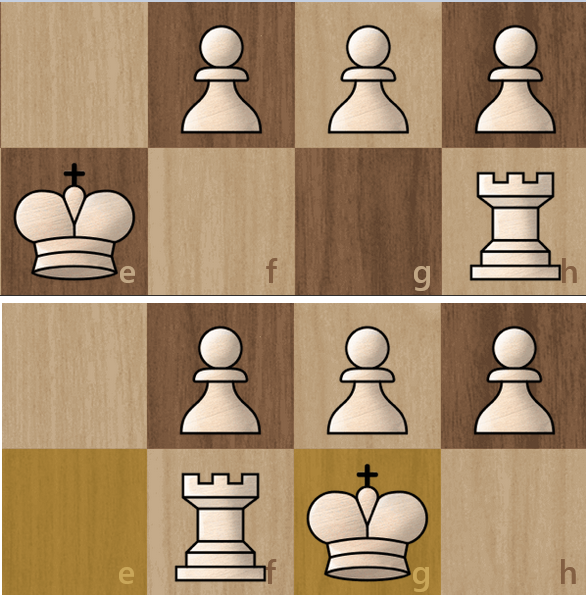
\includegraphics[scale=0.3]{images/rochade.png}
    \caption{Rochade}
\end{figure}

Jeder Zug hat ein Startfeld und ein Endfeld und eine Figur, die sich bewegt. Manche Züge haben jedoch noch weitere Flags. 

\subsubsection{Zug-Flags}
Wenn eine gegnerische Figur geschlagen wird, wird dessen Position in dem \(CAPTURE\) Attribut gespeichert. Dies dient dazu, dass auch bei \(en~passant\) die richtige 
Position der zu schlagenden Figur bekannt ist. Sollte ein Bauer sich zwei Felder vor Bewegen, so wird das neue \(en~passant\) Feld gesetzt, ansonsten wird das alte gelöscht.
Sollte der Bauer auf die letzte Reihe kommen, so wird ein flag gesetzt, welches dies widerspiegelt. 
Bei einer Rochade wird der ein Boolean gesetzt und der Typ der Rochade deklariert. Der Typ variiert hierbei zwischen einer Rochade in Richtung des Damenflügels und Königflügels.

Nach diesen Evaluierungen sind alle vorerst legalen Züge bekannt. Jedoch darf der König nach einem Zug niemals in Schach stehen, also von einer gegnerischen Figur 
angegriffen werden. Um dies zu verhindern, wird bevor der Zug gespeichert wird, er einmal ausgetestet und geprüft, ob der König anschließend angegriffen wird.
Ist das der Fall, wird der Zug aufgrund von Invalidität verworfen, ansonsten ist er legal und wir übernommen.

\subsection{Zug des Spielers}
Wenn der Spieler am Zug ist, kann er entweder über die GUI per drag and drop die gewünschte Figur bewegen, 
oder über die Kamera einen Zug am Brett spielen und diesen einlesen. Der Nutzer kann den Input durch den Button oben rechts in der UI ändern.
Je nach Modus wechselt der Name des Buttons zwischen \(Manual~input\) und \(Video~input\).

\begin{figure}[H]
    \centering
    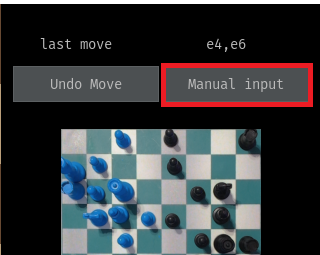
\includegraphics[scale=0.8]{images/manual_camera_input_button.png}
    \caption{Auswahl zwischen manuellem Zug und Kamera}
\end{figure} 

\subsubsection{Manueller Zug}
Die Position des Mauszeigers wird kontinuierlich erfasst. Sollte der Nutzer sich für einen manuellen Zug entscheiden, kann er eine Figur durch Klicken und halten auswählen 
und auf die neue Position ziehen. Die validen Züge werden ihm nun in Grün markiert. Der Zug kann verworfen werden, indem die Figur auf einer invaliden Stelle losgelassen wird 
und durch das Loslassen an einer validen Stelle gezogen werden.
Durch das Loslassen der Figur wird das Feld unter dem Mauszeiger ermittelt und anschließend geprüft, ob es sich hierbei um einen legalen Zug handelt.
Das geschieht, indem die Startposition und Endposition mit denen eines Zuges in der Liste der validen Züge einer Figur übereinstimmen. Wenn das der Fall ist, 
wird dieser Zug als Variable vom Typ \(Move\) zurückgegeben. Das hat den Vorteil, dass so auch die jeweiligen flags in dem Zug verankert sind.

\begin{figure}[H]
    \centering
    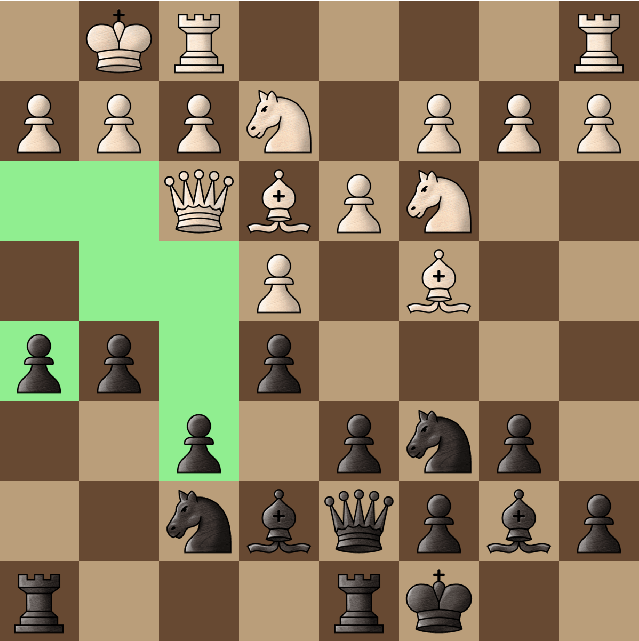
\includegraphics[scale=0.5]{images/manual_input.png}
    \caption{Auswahl zwischen manuellem Zug und Kamera}
\end{figure} 

\subsubsection{Zug durch Bildaufnahme}
Sollte ein Zug per Bildaufnahme getätigt werden, muss der Nutzer zuerst die aktuelle Position abspeichern. 
Das geschieht über das Klicken auf den Knopf \(Capture~position\). Es wäre ebenfalls möglich die aktuelle Position direkt zu speichern, ohne dass der Knopf
betätigt werden muss, jedoch kann dies zu Problemen führen. Wenn der Computergegner einen Zug macht, der eine Figur des Spielers schlägt und der Spieler dann 
den Computerzug nachspielt, anschließend sein eigenen und dann die neue Position aufnimmt, führt dies zu Problemen in der Zugerkennung.
Die Funktionalität ist deshalb so gewählt, dass der Nutzer nach dem Computerzug Zeit hat, diesen Zug zu spielen und anschließend die initiale Position aufzunehmen.

\paragraph{Bildaufnahme}
Der Knopf führt dann die Funktion \(capture\_image()\) von dem \(chessCam\) Objekt aus und speichert das Ergebnis in einer Liste \(positions\).
Die Funktion nutzt dabei die Kamera und liest das aktuelle Bild ein. Dank der vorher ausgewählten Ecken des Schachbretts kann nun eine vier Punkte Transformation 
ausgeführt werden, um nur das Schachbrett aufzunehmen und abzuspeichern.
\begin{figure}[H]
    \centering
    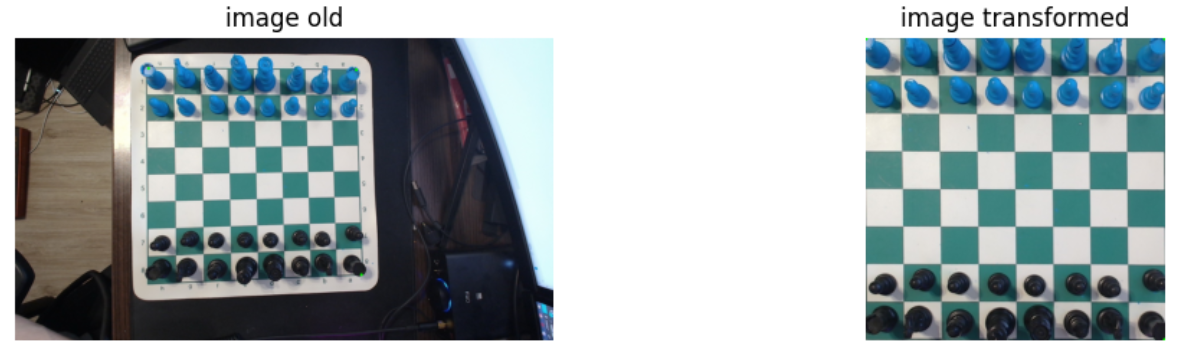
\includegraphics[scale=0.5]{images/transformed_image.png}
    \caption{Vier Punkte Transformation}
\end{figure} 

\paragraph{Zugerkennung}
Nachdem der Nutzer seinen Zug gemacht hat, kann er erneut auf den Knopf drücken und die zweite Position einlesen.
Sobald zwei Positionen eingelesen wurden, wird der Zug ermittelt. Dies geschieht über die Funktion \(get\_move(positions)\).
Diese Funktion des \(chessCam\) Objekts vergleicht die Positionen und gibt den gefundenen Zug als String zurück.

Als Erstes werden die beiden Bilder vorverarbeitet und dadurch die Figuren des Gegners und alle Felder ausmaskiert. Das geschieht über die Werte, die 
der User am Anfang gesetzt hat. Anschließend wird ein Gaußscher Unschärfefilter verwendet, um Unreinheiten zu verwaschen. 
\begin{figure}[H]
    \centering
    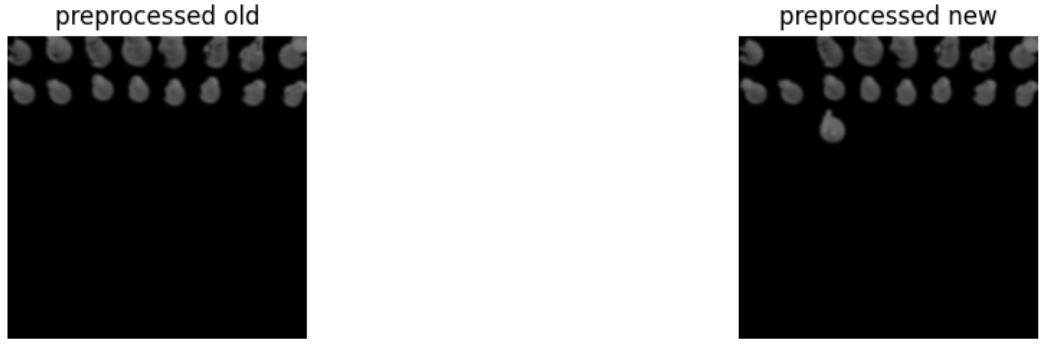
\includegraphics[scale=0.5]{images/preprocessed_image.png}
    \caption{Bildvorverarbeitung}
\end{figure} 

Nachdem die Vorverarbeitung abgeschlossen ist, wird nun die Differenz der beiden Bilder gesucht.
Das geschieht in der Funktion \(compute\_difference(image\_old, image\_new)\). In dieser Funktion wird zunächst der absolute Unterschied zwischen den Bildern 
Pixelweise berechnet. Danach wird ein Schwellenwert auf das erzeugte Bild angewendet. Jeder Pixel dessen Intensität über dem gesetzten Schwellenwert liegt,
wird auf den maximalen Wert gesetzt. Alle anderen Pixel werden auf 0 gesetzt. 
Mithilfe eines Kernels und der OpenCV \(dilate\) Funktion werden weiße Bereiche im Bild vergrößert.
Als Letztes kommt die Erosion, das Gegenstück der \(dilate\) Funktion. Diese Entfernt kleine weiße Pixel. Im Zusammenspiel mit der \(dilate\) Funktion
dient sie dazu, das Rauschen zu verringern.

\begin{figure}[H]
    \centering
    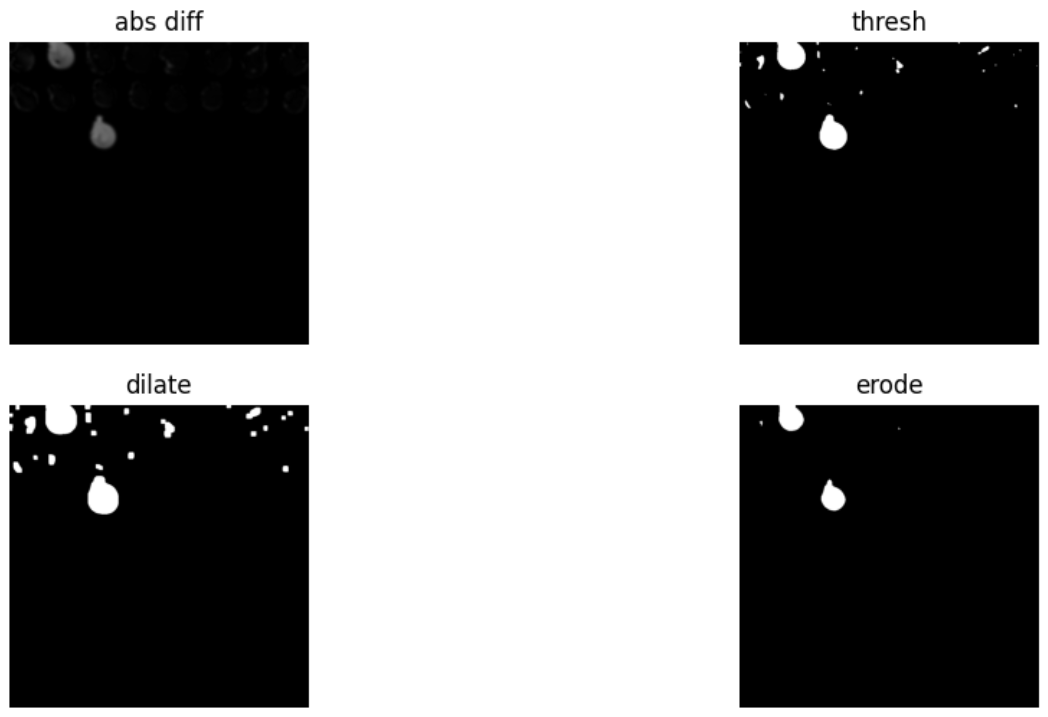
\includegraphics[scale=0.4]{images/compute_difference.png}
    \caption{Berechnung der Unterschiede in den Bildern}
\end{figure} 

Aus dem letzten Bild werden nun die Konturen durch die Funktion \(get\_contours\) extrahiert.  
Die Funktion gibt nur die Konturen und kein Bild zurück. Eine Visualisierung der Konturen würde wie die weiße Umrandung im folgenden Bild aussehen.
\begin{figure}[H]
    \centering
    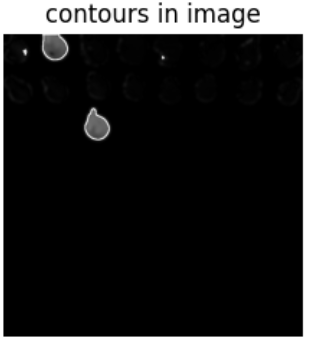
\includegraphics[scale=0.6]{images/contours_in_image.png}
    \caption{Konturen im Bild}
\end{figure} 

Mithilfe dieser Konturen und einer OpenCV Funktion, die dessen Fläche ausrechnet, werden jetzt die Bildunterschiede auf Züge gemappt. 
Dabei wird zunächst ein leeres Array, welches die Züge beinhalten soll, initialisiert. Dann werden alle Konturen durchgegangen und deren Fläche berechnet.
Sollte diese kleiner als ein bestimmter Wert sein, wird sie verworfen. 
Die Iteration über die Konturen wird so lange wiederholt, bis mindestens zwei Züge gefunden werden, oder 500 Iterationen durchgelaufen sind. 
Es ist wichtig, dass nicht auf genau zwei Züge abgefragt wird, da sonst eine Rochade zu Fehlern führen kann.
Bei jeder erneuten Iteration, durch die Konturen wird ein Zähler erhöht. Die Fläche, die eine Kontur braucht, wird mit jeder Iteration exponentiell kleiner und wird 
über eine selbst erstellte Funktion berechnet.

\begin{figure}[H]
    \centering
    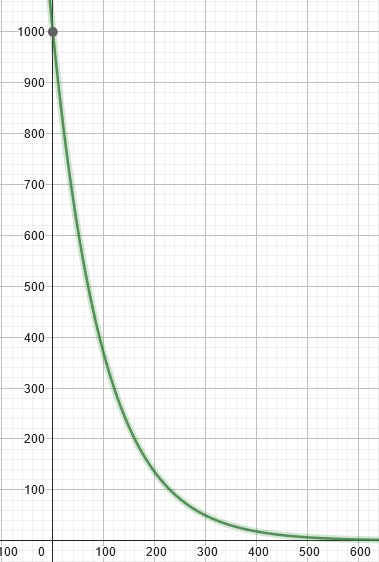
\includegraphics[scale=0.6]{images/contour_area_graph.png}
    \caption{Funktion für die Konturen-Größe $f(x) = 1000 \cdot e^{-0.01x}$}
\end{figure} 

Sollten eine Kontur gefunden werden, ein Rechteck um die Kontur erstellt und dessen Mittelpunkt berechnet. 
Da auf dem Bild nur das Brett zu sehen ist, wird der x- und y-Wert des Mittelpunktes durch die Breite und Höhe eines Feldes, also der \((Breite~oder~Hoehe~des~Bildes)~/ 8\), 
geteilt. Somit kann das genaue Feld auf dem Schachbrett ermittelt werden. 
\begin{figure}[H]
    \centering
    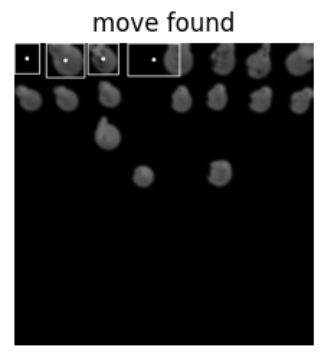
\includegraphics[scale=0.6]{images/move_found.png}
    \caption{Visualisierung des gefundenen Zuges mit Boxen}
\end{figure} 

Der ermittelte Zug wird dann als Liste der veränderten Felder zurückgegeben. Wenn die Länge der Liste zwei beträgt, handelt es sich um keine Rochade.
Nun werden alle Züge durchgegangen, bis ein Zug gefunden wurde, dessen Koordinaten mit den gefundenen übereinstimmen. Wenn das erfolgreich ist, wird der Zug gespielt, 
ansonsten wird der Typ des Inputs auf manuell gesetzt.
Wenn die Länge der Liste vier beträgt, handelt es sich um eine Rochade. Eine Rochade wird als Zug des Königs behandelt mit dem flag \(IS\_CASTLE\).
Es werden also das Start- und Endfeld des Königs herausgefunden und dann ebenfalls ermittelt, ob es sich um einen legalen Zug handelt und dieser dann gespielt.
Sollten weder zwei noch vier Züge erkannt werden, gab es einen Fehler in der Aufnahme und der Typ des Inputs wird ebenfalls auf manuell geschaltet.

Der Spieler kann jederzeit die letzten zwei Züge rückgängig machen, falls ein falscher Zug gespielt wurde. Dabei wird der vorherige Zustand des Schachbretts geladen und
alle Änderungen rückgängig gemacht. Das geht über den Knopf \(Undo~Move\) in der GUI.
\begin{figure}[H]
    \centering
    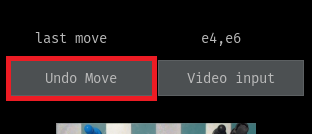
\includegraphics[scale=0.6]{images/undo_move.png}
    \caption{Zug rückgängig machen}
\end{figure} 

\subsection{Zug der Engine}
Wenn die Engine am Zug ist, wird der Zug durch die Funktion \(get\_move()\) ermittelt. Die Engine verwendet dabei die Stockfish Bibliothek und hat eine Wertung von 2000.
Durch die Klasse des Schachbretts wird ein \ac{FEN} String generiert. 

Der \ac{FEN} String ist eine Kurznotation, die jede beliebige Brettstellung widerspiegeln kann.
\(rnbqkbnr/pppppppp/8/8/8/8/PPPPPPPP/RNBQKBNR~w~KQkq~-~0~1\) beschreibt die Startstellung einer Partie. Kleingeschriebene Buchstaben stehen für schwarze die Figuren
und groß geschriebene für die weißen Figuren. Zahlen deuten die Anzahl der leeren Felder an. Schrägstriche leiten eine neue Reihe ein.
Nach den 64 Feldern steht ein Buchstabe für den aktuellen Spieler. Dabei steht \(w\) für weiß und \(b\) für schwarz. \(KQkq\) beschreibt die Rochadenrechte.
Das \(K~und~k\) steht für die Rochade auf dem Königsflügel und das \(Q~und~q\) für die Rochade auf dem Damenflügel, wobei die Groß- und Kleinschreibung wieder die Farbe
repräsentiert. Wenn kein Spieler mehr Rochieren darf, steht stattdessen ein \(-\) anstelle von \(KQkq\). Die vierte Gruppe beschreibt das \(en~passant~Feld\). 
Ein \(-\) zeigt, dass kein \(en~passant\) möglich ist und ein \(a3\) würde ein \(en~passant\) auf dem Feld \(a3\) zulassen.
Die fünfte Gruppe beschreibt die Anzahl der Halbzüge seit dem letzten Bauernzug oder schlagen einer Figur und die sechste Gruppe gibt die nächste Zugnummer an.

Der \ac{FEN} String wird generiert, indem durch das Feld iteriert wird und der Typ der jeweiligen Figur gespeichert wird und 
anschließend die anderen Informationen aus der Schachbrettklasse angehängt werden. Dieser \ac{FEN} String wird dann an die Engine gegeben und diese versucht innerhalb
einer Sekunde den besten Zug zu finden. Dieser Zug wird dann in den validen Zügen gesucht, um ihn als variable vom Typ \(Move\) zurückzugeben und 
anschließend zu spielen.

\subsection{Spielen eines Zuges}
Das Spielen eines Zuges findet in der Funktion \(make\_move(move)\) der Schachbrettklasse statt. Zunächst wird der aktuelle Spielstand gespeichert, damit er
wiederhergestellt werden kann. Im Anschluss wird der Spielzug erhöht, die Farbe des aktuellen Spielers gewechselt, das \(en~passant~Feld\) upgedatet und die Halbzüge
aktualisiert.
Sollte es sich bei dem Zug um eine Rochade handeln, wird eine andere Funktion aufgerufen, die je nach Typ der Rochade die entsprechenden Felder aktualisiert.
Ansonsten wird die gezogene Figur auf dem Spielfeld bewegt und eventuell geschlagene Figuren werden aus dem Array gelöscht.

\begin{figure}[H]
    \centering
    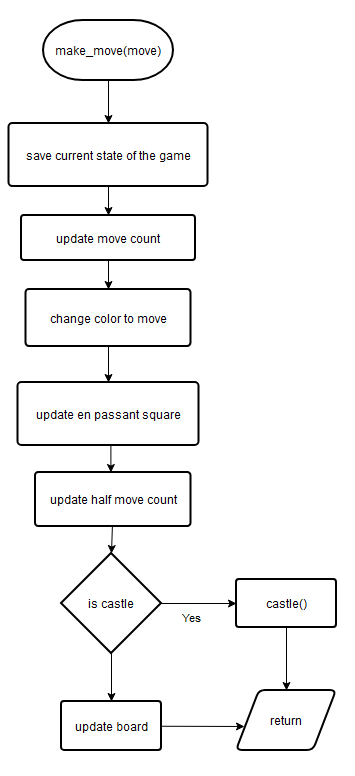
\includegraphics[scale=0.6]{images/make_move_function.png}
    \caption{Funktion zum Spielen eines Zuges}
\end{figure} 

\section{Herausforderungen im Entwicklungsprozess}
Im Verlauf der Entwicklung der Applikation traten ins besondere Probleme bei der Erstellung einer eigenen Schach-Engine und der Kameraauswertung auf.

\subsection{Engine-Entwicklung und Leistung}

\subsubsection{Zeitaufwendige Zugberechnung}
Anfangs wurde versucht eine eigene Engine zu entwickeln. Mit einer einfachen Minimax-Funktion wurden die Suchzeiten jedoch schon bei einer geringen Tiefe 
zu lang. Es wurden diverse Versuche unternommen, die Geschwindigkeit zu verbessern.

\subsubsection{Alpha-Beta-Pruning und andere Lösungen}
Ein weit verbreiteter Ansatz zur Beschleunigung der Minimax-Funktion ist das Alpha-Beta-Pruning. Dies alleine senkte die Rechenzeit der Engine drastisch, jedoch nicht genug,
um sie Nutzen zu können. Andere Optimierungsansätze, wie die Zugsortierung und das Nutzen von Transpositionstabellen hat ebenfalls zu einer nicht ausreichenden 
Leistungssteigerung geführt. Der Hauptgrund dafür ist die Zeit, die der Computer benötigt, um alle legalen Züge einer neuen Position zu berechnen.

\subsubsection{Potenzielle Alternativen}
Lösungsansätze für dieses Problem sind einerseits das Wechseln auf eine effizientere Programmiersprache, oder der Versuch die Funktion an sich effizienter zu machen. 
Beispielsweise ist es statt der Nutzung von Figuren-Objekten in einer Liste, möglich eine Integer-Liste zu nutzen, 
die Anhand ihres Wertes die Farbe, und den Typ der Figur widerspiegeln. Ein weiterer Ansatz ist es, nur die Züge der Figuren zu berechnen, die von dem letzten Zug betroffen 
sind und die anderen Züge beizubehalten. Das Potenzial für die Leistungssteigerung der Funktion ist enorm, jedoch ist die Umsetzung sehr komplex, da zu den eigentlichen Zügen
immer alle betroffenen Figuren ebenfalls berechnet werden müssen. Dies kann die gewonnene Leistungssteigerung stark absenken.

\subsubsection{Verwendung von Stockfish}
In diesem Projekt wurde sich dazu entschieden auf eine externe Engine, Stockfish, zurückzugreifen. Sie ist über eine Python Bibliothek einfach einzubinden und
neben der Leistungssteigerung gehört sie zu den stärksten Engines der Welt.

\subsection{Kamera-Blockaden und irreführende Wahrnehmungen}
Die Nutzung einer Kamera brachte ebenfalls einige Probleme mit sich. Um die Figuren zu erkennen, müssen sich diese deutlich von dem Hintergrund abheben.
Ein erster Ansatz war es, die alte Kamera durch eine Leistungsstärkere auszutauschen, was zu ersten fortschritten geführt hat. Außerdem wurde sich für 
ein Brett entschieden, dessen Farben von den der Figuren abweichen. Dadurch ist es leichter die Figuren auszumaskieren und die Züge mit einer höheren 
Präzision zu finden. Der Winkel der Kamera spielte ebenfalls eine große Rolle. Wenn dieser zu flach war, waren kleinere Figuren hinter größeren versteckt.
Um dieses Problem zu beheben wurde ein Kameraarm montiert, der es erlaubt einen Topdown-View zu erzeugen und die Züge zuverlässig zu finden.




	\chapter{Fazit und Ausblick}
\section{Fazit}
Die Applikation ist im Ganzen ein Erfolg. Die Ziele wurden erreicht, jedoch gab es auch einige Hürden. 
Vor allem im anfänglichen Entwicklungsprozess wurden viele Fehler gemacht und Zeit verschwendet, was verhindert werden konnte. 
Grund dafür war das zu schnelle Starten in die Programmierung ohne ausreichende Vorüberlegungen. Dies führte zu einem Verwerfen vieler 
Arbeit, die dann mehrmals gemacht werden musste. Außerdem, wurde an einigen Stellen, wie der Erstellung einer eigenen Engine viel Zeit verschwendet bei dem 
Versuch durch Optimierung der Suchalgorithmen eine schnellere Suche zu entwickeln, anstatt die Ineffizienz der Zugvalidierung, die der eigentliche 
Auslöser war, anzugehen.  

\section{Ausblick}
\subsection{Online Funktionalität}
Weitere Verbesserungen der Applikation, ist die Verbindung mit Online Portalen, um mit anderen Spielern auf der ganzen Welt spielen zu können.
Im jetzigen Stadium ist es nur möglich gegen eine Engine zu spielen. Mithilfe weiteren Bibliotheken zur Interaktion mit dem Internet oder sogar einem 
eigenen Server kann dies erreicht werden.

\subsection{Speichern der Spiele}
Im jetzigen Stadium der Applikation ist nur das Spielen selber implementiert. Das Abspeichern und anschließende abrufen der Spielzüge erlaubt es dem Nutzer 
sich Fehler wieder anzuschauen und so eine bessere Lernkurve zu erzielen.

\subsection{Spiel auf Zeit}
Schach wird meistens Mithilfe einer Schachuhr gespielt. Diese schränkt die Bedenkzeit beider Spieler ein und bietet eine weitere Herausforderung. Der Grund 
für die noch fehlende Implementierung ist der Zusammenhang mit der Kamera. Wenn der Spieler immer erst den Zug des Gegners spielen muss und dann 
anschließend seinen Zug macht und diesen dann erst über die Kamera aufnimmt, verliert er zu viel Zeit, als dass es Sinn ergibt eine Uhr zu 
implementieren. Durch eine Verbesserung der Zugerkennung, die eventuell automatisch statt manuell läuft, kann dieses Problem umgangen werden.

\subsection{Weitere Spielmodi}
Neben dem klassischen Schach gibt es einige weitere Spaß Modi, die von der Schach-Community gerne gespielt werden. Zurzeit sind diese nicht implementiert aber
vor allem mit Blick auf eine Online Implementation ergibt es Sinn, das Programm um diese zu erweitern.
	
	% Anhang
	\clearpage
	\pagenumbering{roman}

	% Abbildungsverzeichnis
	\cleardoublepage
	\phantomsection \label{listoffig}
	\addcontentsline{toc}{chapter}{Abbildungsverzeichnis}
	\listoffigures

	%Tabellenverzeichnis
	%\cleardoublepage
	%\phantomsection \label{listoftab}
	%\addcontentsline{toc}{chapter}{Tabellenverzeichnis}
	%\listoftables

	% Quellcodeverzeichnis
	%\cleardoublepage
	%\phantomsection \label{listoflist}
	%\addcontentsline{toc}{chapter}{Listings}
	%\lstlistoflistings

	% Literaturverzeichnis
	\cleardoublepage
	\phantomsection \label{listoflit}
	\addcontentsline{toc}{chapter}{Literaturverzeichnis}
	
	%Bib style
	%\bibliographystyle{agsm} %Havard
	\bibliographystyle{ieeetr} %Durchnummeriert
	%\bibliographystyle{amsalpha} %Kürzel für Autor und Jahr
	%see more: http://amath.colorado.edu/documentation/LaTeX/reference/faq/bibstyles.pdf
	
	\bibliography{ArbeitBib}

	% Abkürzungsverzeichnis
	\cleardoublepage
	\phantomsection \label{listofacs}
	\addcontentsline{toc}{chapter}{Abkürzungsverzeichnis}
	%!TEX root = ../dokumentation.tex

\addchap{\langabkverz}
%nur verwendete Akronyme werden letztlich im Abkürzungsverzeichnis des Dokuments angezeigt
%Verwendung: 
%		\ac{Abk.}   --> fügt die Abkürzung ein, beim ersten Aufruf wird zusätzlich automatisch die ausgeschriebene Version davor eingefügt bzw. in einer Fußnote (hierfür muss in header.tex \usepackage[printonlyused,footnote]{acronym} stehen) dargestellt
%		\acs{Abk.}   -->  fügt die Abkürzung ein
%		\acf{Abk.}   --> fügt die Abkürzung UND die Erklärung ein
%		\acl{Abk.}   --> fügt nur die Erklärung ein
%		\acp{Abk.}  --> gibt Plural aus (angefügtes 's'); das zusätzliche 'p' funktioniert auch bei obigen Befehlen
%	siehe auch: http://golatex.de/wiki/%5Cacronym
%	
\begin{acronym}[YTMMM]
\setlength{\itemsep}{-\parsep}

\acro{AGPL}{Affero GNU General Public License}
\acro{WSN}{Wireless Sensor Network}
\acro{MANET}{Mobile wireless Ad-hoc NETwork}
\acro{MAC}{Multiple Access Control}
\acro{QoS}{Quality of Service}
\acro{DSR}{Dynamic Source Routing}
\acro{API}{Application Programming Interface}
\acro{WYSIWYG}{What You See Is What You Get}
\acro{HTML}{HyperText Markup Language}
\acro{Porsche}{Dr. Ing. h.c. F. Porsche AG}
\end{acronym}

	
	% Glossar
	\printglossary[style=altlist,title=Glossar]
\end{document}
